\documentclass[12pt, a4paper]{article}

% 1. Cargar configuraciones
% ============================================================
%  settings.tex --- COPIA ESTO COMPLETO
% ============================================================
\usepackage[utf8]{inputenc}
\usepackage[T1]{fontenc}
\usepackage[spanish,es-noshorthands]{babel}
\usepackage{amsmath, amsfonts, amssymb, amsthm, mathtools, bm, physics}
\usepackage[a4paper, margin=2.5cm]{geometry}
\usepackage{setspace, parskip, microtype, graphicx, booktabs, array, float, caption, xcolor, tcolorbox, enumitem, titlesec, fancyhdr, hyperref}

\tcbuselibrary{theorems, skins, breakable}
\allowdisplaybreaks
\onehalfspacing

% Comandos especiales para fórmulas de las Partes 1 y 4
\newcommand{\E}{\mathbb{E}_t}
\newcommand{\xiit}{\bm{\xi}_t}
\newcommand{\rs}{r^*}
\newcommand{\ns}{n_S}
\newcommand{\nb}{n_B}
\newcommand{\bs}{\beta_S}
\newcommand{\bb}{\beta_B}
\newcommand{\cas}{CA_S}
\newcommand{\cab}{CA_B}

% Encabezados
\pagestyle{fancy}
\fancyhf{}
\rhead{\textit{Macroeconomía Intermedia}}
\lhead{\textsc{Problem Set 1}}
\rfoot{\thepage}

% Definición de Cajas (Usadas en Parte 2 y 3)
\newtcolorbox{resultado}{colback=yellow!10!white, colframe=orange!70!black, fonttitle=\bfseries, title=Resultado, breakable}
\newtcolorbox{condicion}[1][Condición]{colback=blue!5!white, colframe=blue!50!black, fonttitle=\bfseries, title=#1, breakable}
\newtcolorbox{interpretacion}{colback=green!5!white, colframe=green!50!black, fonttitle=\bfseries, title=Interpretación, breakable}
\newtcolorbox{enunciado}{colback=gray!8!white, colframe=gray!50!black, fonttitle=\bfseries, title=Pregunta, breakable}

% 2. Definir los datos del título
\title{
    \textbf{\Huge Macroeconomía Internacional} \\
    \vspace{0.5cm}
    \large Solucionario completo: Problem Set N°1
}
\author{Grupo N°2}

\begin{document}

% 3. Imprimir el título
\maketitle

% --- AQUÍ AGREGAMOS EL MARGEN / ESPACIO EXTRA ---
% Puedes cambiar "2cm" por "3cm" o "1.5cm" según qué tan abajo lo quieras
\vspace{2.5cm} 

% 4. Llamar a los archivos de contenido
\begin{center}
    {\LARGE \textbf{Parte I}}\\[6pt]
\end{center}
\vspace{4pt}\hrule\vspace{10pt}

\subsection*{Ítem 1 }
Definimos el vector de estado $\bm{\xi}_t$ y su rezago $\bm{\xi}_{t-1}$:
\begin{equation}
    \bm{\xi}_t = \begin{bmatrix} y_t \\ y_{t-1} \\ \vdots \\ y_{t-p+1} \end{bmatrix}, \quad \bm{\xi}_{t-1} = \begin{bmatrix} y_{t-1} \\ y_{t-2} \\ \vdots \\ y_{t-p} \end{bmatrix}
\end{equation}
La forma matricial $\bm{\xi}_t = F \bm{\xi}_{t-1} + v_t$ es:
\begin{equation}
    \begin{bmatrix} y_t \\ y_{t-1} \\ \vdots \\ y_{t-p+1} \end{bmatrix} = \begin{bmatrix} 
    \rho_1 & \rho_2 & \dots & \rho_p \\
    1 & 0 & \dots & 0 \\
    \vdots & \vdots & \ddots & \vdots \\
    0 & 0 & 1 & 0
    \end{bmatrix} \begin{bmatrix} y_{t-1} \\ y_{t-2} \\ \vdots \\ y_{t-p} \end{bmatrix} + \begin{bmatrix} \epsilon_t \\ 0 \\ \vdots \\ 0 \end{bmatrix}
\end{equation}
\textbf{Interpretación:} La estabilidad del modelo requiere que los valores propios de F sean menores a 1. Esto garantiza que los efectos de un choque se disipen con el tiempo, evitando que la economía presente un comportamiento explosivo. En términos prácticos, significa que ante un choque de ingresos hoy, su impacto disminuirá gradualmente hasta desaparecer por completo.

\subsection*{Ítem 2 }

Partimos de la ecuación de transición del vector de estado:
\begin{equation}
    \bm{\xi}_t = F \bm{\xi}_{t-1} + v_t
\end{equation}
Para calcular las expectativas de los valores futuros de $\bm{\xi}$ condicionadas a la información disponible en el tiempo $t$ (donde $\E[v_{t+j}] = 0$), realizamos el siguiente proceso iterativo:

\begin{itemize}
    \item \textbf{Para $j=1$:}
    \begin{equation}
        \bm{\xi}_{t+1} = F \bm{\xi}_t + v_{t+1} \implies \E[\bm{\xi}_{t+1}] = F \bm{\xi}_t
    \end{equation}
    
    \item \textbf{Para $j=2$:}
    Usamos el resultado anterior y la propiedad de expectativas iteradas:
    \begin{equation}
        \bm{\xi}_{t+2} = F \bm{\xi}_{t+1} + v_{t+2} \implies \E[\bm{\xi}_{t+2}] = F \E[\bm{\xi}_{t+1}]
    \end{equation}
    Sustituyendo $\E[\bm{\xi}_{t+1}] = F \bm{\xi}_t$:
    \begin{equation}
        \E[\bm{\xi}_{t+2}] = F(F \bm{\xi}_t) = F^2 \bm{\xi}_t
    \end{equation}
\end{itemize}

\textbf{Generalización por Inducción:}
Siguiendo esta lógica para cualquier periodo $j$, llegamos a la solución general:
\begin{equation}
    \E[\bm{\xi}_{t+j}] = F^j \bm{\xi}_t
\end{equation}

\begin{itemize}
    \item \textbf{Interpretación de $F^j$:} Representa el mecanismo de transmisión de la información actual hacia horizontes lejanos. Determina la persistencia de los valores presentes del ingreso y sus rezagos sobre las expectativas futuras después de $j$ períodos.
    
    \item \textbf{Análisis del Límite:} Dado que el sistema es estacionario, cuando $j \to \infty$ se cumple que $F^j \to 0$. Esto implica que la economía disipa el efecto de los choques pasados, permitiendo que las variables converjan a su media de largo plazo. Por tanto, ante un futuro distante, la mejor predicción es que el ingreso retorne a su valor en estado estacionario.
\end{itemize}


\subsection*{Ítem 3}

\textbf{Fórmula de Limpieza de Mercado (Market Clearing):} \\
En equilibrio, el producto total se asigna al consumo, inversión, gasto de gobierno y el saldo neto exterior:
\begin{equation}
    y_t = C_t + i_t + g_t + ca_t
\end{equation}

\textbf{El Problema de Optimización (Lagrangiano):} \\
El hogar busca maximizar el valor esperado de su utilidad cuadrática sujeto a su restricción presupuestaria dinámica. El Lagrangiano ($\mathcal{L}$) se define como:
\begin{equation}
    \mathcal{L} = \E \sum_{j=0}^{\infty} \beta^j \left\{ -\frac{1}{2}(C_{t+j} - \bar{C})^2 + \lambda_{t+j} \left[ y_{t+j} + d_{t+j} - C_{t+j} - (1+r^*)d_{t+j-1} \right] \right\}
\end{equation}
Donde $\lambda_{t+j}$ es el multiplicador de Lagrange (utilidad marginal de la riqueza).

\textbf{Condiciones de Primer Orden (CPO):} \\
Derivamos respecto a las variables de control del hogar ($C_{t+j}$ y $d_{t+j}$):
\begin{enumerate}
    \item \textbf{Respecto al Consumo ($C_{t+j}$):} 
    \begin{equation}
        \frac{\partial \mathcal{L}}{\partial C_{t+j}} = 0 \implies \beta^j [-(C_{t+j} - \bar{C})] - \beta^j \lambda_{t+j} = 0 \implies \bm{\lambda_{t+j} = \bar{C} - C_{t+j}}
    \end{equation}
    \item \textbf{Respecto a la Deuda ($d_{t+j}$):} 
    \begin{equation}
        \frac{\partial \mathcal{L}}{\partial d_{t+j}} = 0 \implies \beta^j \lambda_{t+j} - \E[\beta^{j+1} \lambda_{t+j+1}(1+r^*)] = 0
    \end{equation}
\end{enumerate}

\textbf{Llegada a la Ecuación de Euler:} \\
Sustituyendo la primera CPO en la segunda y utilizando el \textbf{Dato de Calibración} $\beta(1+r^*) = 1$:
\begin{align}
    \lambda_t &= \beta(1+r^*) \E[\lambda_{t+1}] \\
    \lambda_t &= \E[\lambda_{t+1}] \\
    \bar{C} - C_t &= \E[\bar{C} - C_{t+1}] \implies \bm{C_t = \E[C_{t+1}]}
\end{align}

\textbf{Condición de Transversalidad:} \\
Para asegurar que la solución sea óptima en un horizonte infinito, se impone que el valor presente de la deuda sea cero en el límite:
\begin{equation}
    \lim_{j \to \infty} \E \left[ \frac{d_{t+j}}{(1+r^*)^j} \right] = 0
\end{equation}
\textbf{Interpretación:} Esta condición impide que el hogar se endeude infinitamente para consumir hoy (esquema Ponzi) o que muera con una cantidad infinita de activos sin consumir.


\subsection*{Ítem 4}

Partimos de la Condición de Primer Orden (CPO) obtenida en el punto anterior, donde se establece que la utilidad marginal del consumo hoy debe ser igual a la utilidad marginal esperada del mañana:
\begin{equation}
    \lambda_t = \E[\lambda_{t+1}] \implies (\bar{C} - C_t) = \E[\bar{C} - C_{t+1}]
\end{equation}
Simplificando, obtenemos la \textbf{Ecuación de Euler}: $C_t = \E[C_{t+1}]$.

\textbf{Desarrollo Iterativo del Consumo Futuro:} \\
Para demostrar que el nivel de consumo actual es la mejor predicción para cualquier periodo en el futuro, aplicamos el \textbf{Teorema de Expectativas Iteradas} ($\E_t[\E_{t+1}(X)] = \E_t[X]$) paso a paso:

\begin{itemize}
    \item \textbf{Para $j=1$:} 
    Directamente de la ecuación de Euler:
    \begin{equation}
        \E[C_{t+1}] = C_t
    \end{equation}

    \item \textbf{Para $j=2$:} 
    Queremos hallar $\E[C_{t+2}]$. Por la ley de expectativas iteradas, sabemos que:
    \begin{equation}
        \E[C_{t+2}] = \E[ \E_{t+1}(C_{t+2}) ]
    \end{equation}
    Usando la Euler un periodo adelante ($\E_{t+1}[C_{t+2}] = C_{t+1}$), sustituimos:
    \begin{equation}
        \E[C_{t+2}] = \E[C_{t+1}]
    \end{equation}
    Y como ya sabemos que $\E[C_{t+1}] = C_t$, concluimos que:
    \begin{equation}
        \E[C_{t+2}] = C_t
    \end{equation}
\end{itemize}

\textbf{Generalización por Inducción:}
Repitiendo este proceso para cualquier horizonte temporal $j \geq 1$, demostramos que:
\begin{equation}
    \bm{C_t = \E[C_{t+j}]}
\end{equation}

\textbf{Interpretación Económica:}
\begin{itemize}
    \item \textbf{Suavización del Consumo (Consumption Smoothing):} Para evitar que su nivel de vida sea inestable, los hogares recurren al ahorro y al endeudamiento para suavizar su consumo. Esto hace que lo que planeas consumir en el futuro lejano sea igual a lo que consumes hoy. Bajo esta lógica, el consumo se mantiene fijo y solo se ve alterado por noticias totalmente inesperadas o shocks que son imposibles de predecir en el presente.
\end{itemize}

\subsection*{Item 5}

Partimos de la restricción de presupuesto en el periodo $t$: $d_t = (1+r^*)d_{t-1} + C_t - y_t$. 

Despejamos el valor de la deuda inicial:
\begin{equation}
    (1+r^*)d_{t-1} = y_t - C_t + d_t
\end{equation}
Iteramos hacia adelante sustituyendo $d_t$ por su valor esperado en $t+1$, luego $d_{t+1}$ y así sucesivamente:
\begin{align}
    (1+r^*)d_{t-1} &= (y_t - C_t) + \E \left[ \frac{y_{t+1} - C_{t+1} + d_{t+1}}{1+r^*} \right] \\
    (1+r^*)d_{t-1} &= (y_t - C_t) + \frac{\E[y_{t+1} - C_{t+1}]}{1+r^*} + \frac{\E[y_{t+2} - C_{t+2}]}{(1+r^*)^2} + \dots + \frac{\E[d_{t+j}]}{(1+r^*)^j}
\end{align}

Aplicando el límite de la \textbf{Condición de Transversalidad (No-Ponzi Scheme)}: $\lim_{j \to \infty} \E \left[ \frac{d_{t+j}}{(1+r^*)^j} \right] = 0$, obtenemos la Ecuación 9:
\begin{equation}
    (1+r^*)d_{t-1} = \E \sum_{j=0}^{\infty} \frac{y_{t+j} - C_{t+j}}{(1+r^*)^j}
\end{equation}

\subsection*{Item 6}


Partimos de la Restricción Presupuestaria Intertemporal obtenida en el punto anterior (Ecuación 9):
\begin{equation}
    (1+r^*)d_{t-1} = \E \sum_{j=0}^{\infty} \frac{y_{t+j} - C_{t+j}}{(1+r^*)^j}
\end{equation}

\textbf{Paso 1: Separación de la sumatoria.} \\
Aplicamos la propiedad de linealidad de la esperanza y de las sumatorias para separar el ingreso del consumo:
\begin{equation}
    (1+r^*)d_{t-1} = \E \sum_{j=0}^{\infty} \frac{y_{t+j}}{(1+r^*)^j} - \E \sum_{j=0}^{\infty} \frac{C_{t+j}}{(1+r^*)^j}
\end{equation}

\textbf{Paso 2: Aplicación de la Suavización del Consumo.} \\
Por la Ecuación de Euler y el Teorema de Expectativas Iteradas (Punto 4), sabemos que $\E[C_{t+j}] = C_t$ para todo $j \geq 0$. Sustituimos esto en la segunda sumatoria:
\begin{equation}
    \E \sum_{j=0}^{\infty} \frac{C_{t+j}}{(1+r^*)^j} = \sum_{j=0}^{\infty} \frac{C_t}{(1+r^*)^j} = C_t \sum_{j=0}^{\infty} \left( \frac{1}{1+r^*} \right)^j
\end{equation}

\textbf{Paso 3: Resolución de la Serie Geométrica Infinita.} \\
Recordamos que una serie de la forma $\sum_{j=0}^{\infty} a^j$ converge a $\frac{1}{1-a}$ si $|a| < 1$. En nuestro caso, $a = \frac{1}{1+r^*}$:
\begin{equation}
    \sum_{j=0}^{\infty} \left( \frac{1}{1+r^*} \right)^j = \frac{1}{1 - \frac{1}{1+r^*}} = \frac{1}{\frac{1+r^*-1}{1+r^*}} = \frac{1+r^*}{r^*}
\end{equation}

\textbf{Paso 4: Sustitución y Despeje de $C_t$.} \\
Sustituimos el resultado de la serie en la ecuación principal:
\begin{equation}
    (1+r^*)d_{t-1} = \E \sum_{j=0}^{\infty} \frac{y_{t+j}}{(1+r^*)^j} - C_t \left( \frac{1+r^*}{r^*} \right)
\end{equation}
Ahora, despejamos el término que contiene al consumo:
\begin{equation}
    C_t \left( \frac{1+r^*}{r^*} \right) = \E \sum_{j=0}^{\infty} \frac{y_{t+j}}{(1+r^*)^j} - (1+r^*)d_{t-1}
\end{equation}
Multiplicamos toda la ecuación por $\left( \frac{r^*}{1+r^*} \right)$ para aislar $C_t$:
\begin{equation}
    C_t = \left( \frac{r^*}{1+r^*} \right) \E \sum_{j=0}^{\infty} \frac{y_{t+j}}{(1+r^*)^j} - \left( \frac{r^*}{1+r^*} \right) (1+r^*)d_{t-1}
\end{equation}

\textbf{Resultado Final (Ecuación 10):}
\begin{equation}
    C_t = \underbrace{\frac{r^*}{1+r^*} \E \sum_{j=0}^{\infty} \frac{y_{t+j}}{(1+r^*)^j}}_{\text{Riqueza Humana (Anualizada)}} - \underbrace{r^* d_{t-1}}_{\text{Riqueza Financiera (Servicio)}}
\end{equation}

\textbf{Interpretación:} El consumo de hoy no depende de si recibiste un bono hoy o si disminuye tu salario (ingreso transitorio), sino de tu ingreso permanente. Si recibes \$1000 hoy, solo consumes $r^* \times 1000$ y ahorras el resto para mantener ese nivel de consumo cuando ya no tengas el cheque. Solo gastas los intereses que ese dinero te daría por el resto de tu vida.

\subsection*{ítem 7}

Partimos de la definición de la Cuenta Corriente: $ca_t = y_t - C_t - r^*d_{t-1}$. El objetivo es demostrar cómo el saldo externo depende de las expectativas de cambios futuros en el ingreso.

\textbf{Paso 1: Sustitución del Consumo ($C_t$).} \\
Sustituimos la Ecuación 10 en la definición de $ca_t$:
\begin{equation}
    ca_t = y_t - \left[ \frac{r^*}{1+r^*} \E \sum_{j=0}^{\infty} \frac{y_{t+j}}{(1+r^*)^j} - r^* d_{t-1} \right] - r^* d_{t-1}
\end{equation}
Notamos que los términos de riqueza financiera (deuda) $-(-r^* d_{t-1})$ y $-r^* d_{t-1}$ se cancelan exactamente:
\begin{equation}
    ca_t = y_t - \frac{r^*}{1+r^*} \E \sum_{j=0}^{\infty} \frac{y_{t+j}}{(1+r^*)^j}
\end{equation}

\textbf{Paso 2: Desglose del primer término de la sumatoria ($j=0$).} \\
Extraemos el ingreso actual ($y_t$) de la sumatoria infinita:
\begin{equation}
    ca_t = y_t - \frac{r^*}{1+r^*} \left[ y_t + \E \sum_{j=1}^{\infty} \frac{y_{t+j}}{(1+r^*)^j} \right]
\end{equation}
Agrupamos los términos que contienen $y_t$:
\begin{equation}
    ca_t = y_t \left( 1 - \frac{r^*}{1+r^*} \right) - \frac{r^*}{1+r^*} \E \sum_{j=1}^{\infty} \frac{y_{t+j}}{(1+r^*)^j}
\end{equation}
Simplificando el paréntesis: $1 - \frac{r^*}{1+r^*} = \frac{1+r^*-r^*}{1+r^*} = \frac{1}{1+r^*}$. Obtenemos:
\begin{equation}
    ca_t = \frac{y_t}{1+r^*} - \frac{r^*}{1+r^*} \E \sum_{j=1}^{\infty} \frac{y_{t+j}}{(1+r^*)^j}
\end{equation}

\textbf{Paso 3: Transformación a Variaciones ($\Delta y$).} \\
Utilizamos el hecho de que $y_t$ puede expresarse como una serie geométrica ponderada por sus propios cambios futuros. Mediante manipulación algebraica de los términos $y_{t+j}$, reescribimos la ecuación en función de $\Delta y_{t+j} = y_{t+j} - y_{t+j-1}$:
\begin{equation}
    ca_t = -\E \sum_{j=1}^{\infty} \frac{\Delta y_{t+j}}{(1+r^*)^j}
\end{equation}

\textbf{Interpretación:} " Ahorras para un día lluvioso". Si esperas que el ingreso baje en el futuro ($\Delta y < 0$), ahorras hoy ($ca_t > 0$). Tu cuenta corriente entra en superavit. Por el otro lado, si tu ingreso sube ($\Delta y > 0$). Eres más rico en el futuro, pides prestado hoy para empezar a vivir bien. Tu cuenta corriente entra déficit.  

\subsection*{ítem 8}

\textbf{Reescribiendo la Ecuación 10 (Consumo e Ingreso Permanente):} \\
Sabemos que $y_t^p = \frac{r^*}{1+r^*} \E \sum_{j=0}^{\infty} \frac{y_{t+j}}{(1+r^*)^j}$. Para llevar esto a su forma matricial, usamos que $y_{t+j} = \mathbf{e}_1^\top \bm{\xi}_{t+j}$ y que $\E[\bm{\xi}_{t+j}] = F^j \bm{\xi}_t$:

\begin{align}
    y_t^p &= \frac{r^*}{1+r^*} \sum_{j=0}^{\infty} \frac{\mathbf{e}_1^\top F^j \bm{\xi}_t}{(1+r^*)^j} \\
    y_t^p &= \left[ \frac{r^*}{1+r^*} \mathbf{e}_1^\top \sum_{j=0}^{\infty} \left( \frac{F}{1+r^*} \right)^j \right] \bm{\xi}_t
\end{align}

Usando la propiedad de la serie geométrica matricial $\sum_{j=0}^{\infty} M^j = (I - M)^{-1}$, definimos el vector de coeficientes $\bm{\Gamma}^\top$:
\begin{equation}
    \bm{\Gamma}^\top = \frac{r^*}{1+r^*} \mathbf{e}_1^\top \left( I_p - \frac{F}{1+r^*} \right)^{-1}
\end{equation}
Por lo tanto, la ecuación reescrita es: $\bm{y_t^p = \bm{\Gamma}^\top \bm{\xi}_t}$.

\vspace{1em}
\vspace{1em}
\textbf{Reescribiendo la Ecuación 10 (Hacia el Ingreso Permanente Matricial)} \\
Partimos de la definición teórica del consumo:
\begin{equation}
    C_t = \frac{r^*}{1+r^*} \E \sum_{j=0}^{\infty} \frac{y_{t+j}}{(1+r^*)^j} - r^* d_{t-1}
\end{equation}
Para operarlo matricialmente, definimos el \textbf{Ingreso Permanente} ($y_t^p$) como la anualidad de la riqueza humana. Usamos la propiedad $y_{t+j} = \mathbf{e}_1^\top \bm{\xi}_{t+j}$ y la predicción $\E[\bm{\xi}_{t+j}] = F^j \bm{\xi}_t$:

\begin{enumerate}
    \item \textbf{Sustitución:} 
    $y_t^p = \frac{r^*}{1+r^*} \sum_{j=0}^{\infty} \frac{\mathbf{e}_1^\top F^j \bm{\xi}_t}{(1+r^*)^j}$
    \item \textbf{Factorización del vector de estado:} Sacamos los términos constantes de la sumatoria:
    $y_t^p = \left[ \frac{r^*}{1+r^*} \mathbf{e}_1^\top \sum_{j=0}^{\infty} \left( \frac{F}{1+r^*} \right)^j \right] \bm{\xi}_t$
    \item \textbf{Solución de la serie de potencias:} Como los valores propios de $F$ están dentro del círculo unitario, la serie converge a $(I - M)^{-1}$:
    $\bm{\Gamma}^\top = \frac{r^*}{1+r^*} \mathbf{e}_1^\top \left( I_p - \frac{F}{1+r^*} \right)^{-1}$
\end{enumerate}

\textbf{Resultado Final:}
\begin{equation}
    C_t = \underbrace{\bm{\Gamma}^\top \bm{\xi}_t}_{y_t^p} - r^* d_{t-1}
\end{equation}

\textbf{Interpretación del proceso:} 
Al reescribir la ecuación de esta manera, demostramos que el consumo no solo depende del ingreso observado hoy ($y_t$), sino de toda la información contenida en el vector de estado $\bm{\xi}_t$ (que incluye los rezagos del ingreso). Esto permite que el agente asigne ponderaciones ($\bm{\Gamma}^\top$) a cada dato pasado para predecir su riqueza futura y decidir su nivel de vida actual.

\textbf{Cuenta Corriente (Ecuacion 11):} \\
Partimos de $ca_t = -\E \sum_{j=1}^{\infty} \frac{\Delta y_{t+j}}{(1+r^*)^j}$. Sabiendo que $\Delta y_{t+j} = y_{t+j} - y_{t+j-1} = \mathbf{e}_1^\top (F^j - F^{j-1}) \bm{\xi}_t$:

\begin{equation}
    ca_t = -\mathbf{e}_1^\top \left[ \sum_{j=1}^{\infty} \frac{F^j - F^{j-1}}{(1+r^*)^j} \right] \bm{\xi}_t
\end{equation}

Factorizando y simplificando la serie matricial, obtenemos la forma compacta:
\begin{equation}
    ca_t = \mathbf{e}_1^\top \left[ I_p - \left( I_p - \frac{F}{1+r^*} \right)^{-1} \right] \bm{\xi}_t
\end{equation}

\subsection*{Análisis Final: Invertibilidad y Relaciones Económicas}

\textbf{1. ¿Por qué es invertible la matriz $(I_p - \frac{F}{1+r^*})$?} \\
La invertibilidad de esta matriz es fundamental para hallar la solución del ingreso permanente. Matemáticamente, se garantiza por dos razones:
\begin{itemize}
    \item \textbf{Condición de Estacionariedad:} Por dato, el proceso del ingreso es estacionario, lo que implica que todos los valores propios ($\lambda$) de la matriz compañera $F$ son menores a 1 en valor absoluto ($|\lambda| < 1$).
    \item \textbf{Factor de Descuento:} Dado que $r^* > 0$, el término $\frac{1}{1+r^*}$ es menor a 1. Por lo tanto, los valores propios de la matriz modificada $\frac{F}{1+r^*}$ son aún más pequeños. 
    \item \textbf{Conclusión:} Como ningún valor propio de $\frac{F}{1+r^*}$ puede ser igual a 1, la matriz $(I_p - \frac{F}{1+r^*})$ es no singular (su determinante es distinto de cero) y, por lo tanto, su inversa existe.
\end{itemize}

\textbf{2. Relación entre el Ingreso Actual ($y_t$) y el Ingreso Permanente ($y_t^p$)} \\
Esta relación define la posición financiera del país o individuo:
\begin{itemize}
    \item \textbf{Si $y_t > y_t^p$ (Acreedor Neto):} El ingreso observado hoy es superior al promedio de ingresos que esperas recibir durante el resto de tu vida. Esto se considera un auge temporal. Para mantener el consumo estable en el futuro, el agente debe ahorrar el excedente hoy.
    \item \textbf{Si $y_t < y_t^p$ (Deudor Neto):} El ingreso actual es inferior al promedio de vida. Para no bajar su nivel de vida (suavización del consumo), el agente pide prestado contra sus ingresos futuros.
\end{itemize}

\textbf{3. Interpretación Final de la Cuenta Corriente ($ca_t$)} \\
La ecuación $ca_t = -\E \sum_{j=1}^{\infty} \frac{\Delta y_{t+j}}{(1+r^*)^j}$ nos da la clave del sector externo:
\begin{itemize}
    \item \textbf La cuenta corriente actúa como un amortiguador. Si el agente anticipa que sus ingresos futuros van a caer ($\Delta y < 0$), la sumatoria se vuelve negativa, y debido al signo menos exterior, la $ca_t$ resulta positiva. 
    \item \textbf{Resultado:} Un superávit en la cuenta corriente hoy es la señal de que el país se está preparando para una disminución futura de sus recursos.
\end{itemize}

 \newpage
\begin{center}
    {\LARGE \textbf{Parte II}}\\[6pt]
\end{center}
\vspace{4pt}\hrule\vspace{10pt}

% ==================================================================
\section*{Item 9}
% ==================================================================

\begin{enunciado}
Demostrar que:
\[
    \frac{\partial y_{t+j}}{\partial \varepsilon_t} = f_{11}^{(j)}
\]
donde $f_{11}^{(j)}$ es el elemento $(1,1)$ de $F^j$.
\end{enunciado}

\subsection*{Solucion}

\paragraph{Paso 1: Identidad de partida.}
Partimos de la identidad:
\[
    Y_{t+j} = \mathbf{e}_1^T \xi_{t+j}
\]

\paragraph{Paso 2: Derivar el vector de estados respecto a $\varepsilon_t$.}

Tomamos el vector de estados $\xi_t = F\xi_{t-1} + \mathbf{v}_t$ y derivamos respecto a $\varepsilon_t$:
\[
    \frac{\partial \xi_t}{\partial \varepsilon_t}
    = \frac{\partial (F\xi_{t-1} + \mathbf{v}_t)}{\partial \varepsilon_t}
\]

Separamos los dos terminos:
\[
    \frac{\partial \xi_t}{\partial \varepsilon_t}
    = \frac{\partial F\xi_{t-1}}{\partial \varepsilon_t} + \frac{\partial \mathbf{v}_t}{\partial \varepsilon_t}
\]

El primer termino es cero porque $\xi_{t-1}$ ya ocurrio antes del shock, por lo tanto es independiente de $\varepsilon_t$:
\[
    \frac{\partial \xi_{t-1}}{\partial \varepsilon_t} = 0
\]

Entonces nos queda:
\[
    \frac{\partial \xi_t}{\partial \varepsilon_t} = \frac{\partial \mathbf{v}_t}{\partial \varepsilon_t}
\]

\paragraph{Paso 3: Calcular $\partial \mathbf{v}_t / \partial \varepsilon_t$.}

Recordamos que el vector de perturbaciones tiene la forma:
\[
    \mathbf{v}_t = \begin{pmatrix} \varepsilon_t \\ 0 \\ \vdots \\ 0 \end{pmatrix}
\]

Podemos factorizar $\varepsilon_t$:
\[
    \mathbf{v}_t = \varepsilon_t \cdot \begin{pmatrix} 1 \\ 0 \\ 0 \\ \vdots \\ 0 \end{pmatrix}
    = \varepsilon_t \cdot \mathbf{e}_1
\]

Entonces derivando respecto a $\varepsilon_t$:
\[
    \frac{\partial \mathbf{v}_t}{\partial \varepsilon_t}
    = \frac{\partial (\varepsilon_t \cdot \mathbf{e}_1)}{\partial \varepsilon_t}
    = \mathbf{e}_1
\]

Por tanto:
\[
    \frac{\partial \xi_t}{\partial \varepsilon_t} = \mathbf{e}_1
\]

\paragraph{Paso 4: Derivar $Y_{t+j}$ respecto a $\varepsilon_t$.}

Partimos de la identidad y derivamos:
\[
    \frac{\partial Y_{t+j}}{\partial \varepsilon_t}
    = \frac{\partial \mathbf{e}_1^T \xi_{t+j}}{\partial \varepsilon_t}
\]

Usando la ecuacion (7), que nos dice que $\mathbb{E}_t[\xi_{t+j}] = F^j \xi_t$, aplicamos la regla de la cadena:
\[
    \frac{\partial Y_{t+j}}{\partial \varepsilon_t}
    = \mathbf{e}_1^T F^j \frac{\partial \xi_t}{\partial \varepsilon_t}
\]

Dado que tambien $\partial \xi_{t-1}/\partial \varepsilon_t = 0$, la derivada de $\xi_t$ es simplemente $\mathbf{e}_1$. Sustituyendo:
\[
    \frac{\partial Y_{t+j}}{\partial \varepsilon_t}
    = \mathbf{e}_1^T F^j \mathbf{e}_1
\]

\paragraph{Paso 5: Extraer el elemento $(1,1)$.}

Recordamos que:
\[
    \mathbf{e}_1 = \begin{pmatrix} 1 \\ 0 \\ \vdots \\ 0 \end{pmatrix}
    \qquad \text{y} \qquad
    F^j = \begin{pmatrix} f_{11}^{(j)} & f_{12}^{(j)} & \cdots \\ f_{21}^{(j)} & f_{22}^{(j)} & \cdots \\ \vdots & & \ddots \end{pmatrix}
\]

Calculamos $F^j \mathbf{e}_1$: multiplicar $F^j$ por $\mathbf{e}_1$ extrae la primera columna de $F^j$:
\[
    F^j \mathbf{e}_1 = \begin{pmatrix} f_{11}^{(j)} \\ f_{21}^{(j)} \\ \vdots \end{pmatrix}
\]

Ahora multiplicamos por $\mathbf{e}_1^T$ por la izquierda, lo que extrae unicamente el primer elemento del vector:
\[
    \mathbf{e}_1^T \begin{pmatrix} f_{11}^{(j)} \\ f_{21}^{(j)} \\ \vdots \end{pmatrix}
    = f_{11}^{(j)}
\]

\begin{resultado}
\[
    \frac{\partial y_{t+j}}{\partial \varepsilon_t} = f_{11}^{(j)}
\]
La IRF del ingreso es simplemente el elemento $(1,1)$ de la potencia $j$-esima de la matriz companera $F$.
\end{resultado}

% ==================================================================
\section*{Ítem 10}
% ==================================================================

\begin{enunciado}
Tomando en cuenta que $f_{11}^{(j)} = c_1\lambda_1^j + \cdots + c_p\lambda_p^j$ (suma de valores propios de $F$), demostrar las condiciones bajo las cuales la IRF es \textit{hump-shaped}.
\end{enunciado}

\subsection*{Solucion}

\paragraph{i) Condicion para IRF hump-shaped.}

La IRF es \textit{hump-shaped} si la respuesta de $Y$ ante el shock no es maxima en el momento en que ocurre el shock, sino que primero aumenta durante varios periodos, alcanza un pico en algun horizonte $j^* > 0$ y luego comienza a decrecer hasta converger a cero. Formalmente:
\[
    f_{11}^{(0)} < f_{11}^{(j^*)}, \quad \text{para algun } j^* \geq 1
\]

La condicion para que esto ocurra es que los valores propios de $F$ sean \textbf{numeros complejos}:
\[
    \lambda_i = a \pm bi \quad \text{con } b \neq 0
\]

\paragraph{Razon: forma polar de valores propios complejos.}

Cuando los valores propios son complejos se pueden expresar en forma polar:
\[
    \lambda = |r| e^{i\theta}
    \quad \text{donde} \quad
    |r| = \sqrt{a^2 + b^2}, \quad
    \theta = \arctan\!\left(\frac{b}{a}\right)
\]

Elevando a la potencia $j$:
\[
    \lambda^j = |r|^j e^{ij\theta}
\]

Aplicando la formula de Euler $e^{i\theta} = \cos\theta + i\sin\theta$:
\[
    \lambda^j = |r|^j \bigl(\cos(j\theta) + i\sin(j\theta)\bigr)
\]

Recordamos que $\cos(j\theta)$ oscila entre $-1$ y $1$ dependiendo del angulo.

\paragraph{Suma de pares conjugados.}

Los valores propios complejos vienen en pares conjugados:
\[
    \lambda_i = a + bi, \qquad \bar{\lambda}_i = a - bi
\]

Sumando su contribucion a $f_{11}^{(j)}$:
\[
    c_i \lambda_i^j + c_{i+1} \bar{\lambda}_i^j
    = r^j(\cos(j\theta) + i\sin(j\theta)) + r^j(\cos(j\theta) - i\sin(j\theta))
\]
\[
    = 2|r|^j \cos(j\theta)
\]

Si $\theta$ es pequeno, el coseno empieza cerca de 1 y sube lentamente antes de bajar, generando la joroba.

\paragraph{Por que no pueden ser reales.}

\begin{itemize}
    \item \textbf{Todos reales positivos:} la IRF solo decreceria monotonamente desde el impacto, sin formar joroba.
    \item \textbf{Todos reales negativos:} los valores propios alternan entre positivos y negativos de manera brusca (ver tabla):
\end{itemize}

\begin{center}
\begin{tabular}{cc}
\hline
$j$ & $\lambda^j$ (con $\lambda = -0.8$) \\
\hline
0 & 1 \\
1 & $-0.8$ \\
2 & $0.64$ \\
3 & $-0.51$ \\
\hline
\end{tabular}
\end{center}

Esta alternancia brusca no genera una joroba suave.

\begin{resultado}
La condicion necesaria para una IRF \textit{hump-shaped} es que la matriz $F$ tenga al menos un par de valores propios \textbf{complejos conjugados} $\lambda = a \pm bi$ con $b \neq 0$ y $|r| < 1$.
\end{resultado}

\paragraph{ii) Relevancia para la cuenta corriente.}

Recordamos la ecuacion de la cuenta corriente (11):
\[
    ca_t = -\mathbb{E}_t \sum_{j=1}^{\infty} \frac{\Delta y_{t+j}}{(1+r^*)^j}
\]

La cuenta corriente depende de los cambios esperados del ingreso futuro.

Con una IRF \textit{hump-shaped} tras el shock $\varepsilon_t$:

\begin{itemize}
    \item \textbf{Fase ascendente} ($0 \leq j < j^*$): el ingreso sigue subiendo y aun no llega al pico ($f_{11}^{(0)} < f_{11}^{(j^*)}$). Como el consumidor sabe que aun no ha llegado al nivel maximo, consume mas de lo que produce y se endeuda.
    \item \textbf{En el pico} ($j = j^*$): el ingreso empieza a bajar; el consumidor sabe que en adelante tendra menos, por lo que suaviza el consumo y empieza a pagar deuda.
    \item \textbf{Fase descendente} ($j > j^*$): el ingreso sigue por encima del consumo, hay superavit y se paga deuda.
\end{itemize}

% ==================================================================
\section*{ítem 11}
% ==================================================================

\subsection*{i) Demostrar que $\dfrac{\partial y_{t+j}^p}{\partial \varepsilon_t} = \Gamma^T F^j e_1$}

\begin{enunciado}
\[
    \frac{\partial y_{t+j}^p}{\partial \varepsilon_t} = \Gamma^T F^j e_1
\]
\end{enunciado}

\paragraph{Solucion.}

Del item (8) tenemos la definicion del ingreso permanente:
\[
    y_t^p = \Gamma^T \xi_t
\]
donde $\xi_t$ es el vector de estados y $\Gamma^T$ es el vector de pesos de descuento.

Derivamos respecto a $\varepsilon_t$:
\[
    \frac{\partial y_{t+j}^p}{\partial \varepsilon_t}
    = \Gamma^T \frac{\partial \xi_{t+j}}{\partial \varepsilon_t}
\]

Del Ejercicio 9 sabemos que:
\[
    \frac{\partial \xi_{t+j}}{\partial \varepsilon_t} = F^j e_1
\]

Sustituyendo directamente:
\[
    \frac{\partial y_{t+j}^p}{\partial \varepsilon_t} = \Gamma^T F^j e_1
\]

\begin{resultado}
\[
    \frac{\partial y_{t+j}^p}{\partial \varepsilon_t} = \Gamma^T F^j e_1
\]
\textbf{Interpretacion:} Esta expresion indica cuanto cambiara el ingreso permanente $j$ periodos despues del shock $\varepsilon_t$. $\Gamma^T$ acumula una suma ponderada de las respuestas futuras. Si el shock es permanente, $F^j e_1$ se mantiene grande y $\Gamma^T$ acumula una suma alta $\Rightarrow$ el ingreso permanente sube mucho. Si el shock es transitorio, $F^j e_1$ cae rapido y la suma es pequena.
\end{resultado}

\subsection*{ii) Demostrar que $\dfrac{\partial ca_{t+j}}{\partial \varepsilon_t} = (\mathbf{e}_1^T - \Gamma^T) F^j e_1$}

\begin{enunciado}
\[
    \frac{\partial ca_{t+j}}{\partial \varepsilon_t} = (\mathbf{e}_1^T - \Gamma^T) F^j e_1
\]
\end{enunciado}

\paragraph{Paso 1: Expresar $c_t$ en terminos del ingreso permanente.}

Partimos de la ecuacion (10):
\[
    c_t = \frac{r^*}{1+r^*} \mathbb{E}_t \sum_{j=0}^{\infty} \frac{y_{t+j}}{(1+r^*)^j} - r^* d_{t-1}
\]

Del item (8) reconocemos que:
\[
    y_t^p \equiv \frac{r^*}{1+r^*} \mathbb{E}_t \sum_{j=0}^{\infty} \frac{y_{t+j}}{(1+r^*)^j}
\]

Entonces podemos reescribir el consumo como:
\[
    c_t = y_t^p - r^* d_{t-1}
\]

\paragraph{Paso 2: Sustituir en la cuenta corriente.}

De la ecuacion (5):
\[
    ca_t = y_t - c_t - r^* d_{t-1}
\]

Sustituimos $c_t = y_t^p - r^* d_{t-1}$:
\[
    ca_t = y_t - (y_t^p - r^* d_{t-1}) - r^* d_{t-1}
\]

Expandimos el parentesis:
\[
    ca_t = y_t - y_t^p + r^* d_{t-1} - r^* d_{t-1}
\]

Los terminos $r^* d_{t-1}$ se cancelan:
\[
    \boxed{ca_t = y_t - y_t^p}
\]

La cuenta corriente es la diferencia entre el ingreso corriente y el ingreso permanente.

\paragraph{Paso 3: Derivar respecto a $\varepsilon_t$.}

\[
    \frac{\partial ca_{t+j}}{\partial \varepsilon_t}
    = \frac{\partial y_{t+j}}{\partial \varepsilon_t} - \frac{\partial y_{t+j}^p}{\partial \varepsilon_t}
\]

Por el Ejercicio 9 (ecuacion 14):
\[
    \frac{\partial y_{t+j}}{\partial \varepsilon_t} = \mathbf{e}_1^T F^j e_1
\]

Por el item anterior (ecuacion 16):
\[
    \frac{\partial y_{t+j}^p}{\partial \varepsilon_t} = \Gamma^T F^j e_1
\]

Sustituyendo ambos:
\[
    \frac{\partial ca_{t+j}}{\partial \varepsilon_t}
    = \mathbf{e}_1^T F^j e_1 - \Gamma^T F^j e_1
\]

Factorizamos $F^j e_1$:

\begin{resultado}
\[
    \frac{\partial ca_{t+j}}{\partial \varepsilon_t} = (\mathbf{e}_1^T - \Gamma^T) F^j e_1
\]
\end{resultado}

\paragraph{Rol de $(\mathbf{e}_1^T - \Gamma^T)$.}

\begin{condicion}[Shock transitorio]
$\mathbf{e}_1^T F^j e_1 > \Gamma^T F^j e_1$ porque el ingreso corriente sube mas que el permanente. La brecha $\mathbf{e}_1^T - \Gamma^T > 0$ implica superavit: el hogar consume menos de lo que produce.
\end{condicion}

\begin{condicion}[Shock permanente]
$\mathbf{e}_1^T F^j e_1 = \Gamma^T F^j e_1$ porque el ingreso corriente y permanente suben igual. La diferencia es cero: no hay superavit ni deficit.
\end{condicion}

% ==================================================================
\section*{Ítem 12}
% ==================================================================

\subsection*{i) Demostrar que $\displaystyle\sum_{j=0}^{T} \dfrac{\partial ca_{t+j}}{\partial \varepsilon_t} = -\dfrac{\partial d_{t+T}}{\partial \varepsilon_t}$}

\paragraph{Paso 1: Iterar la restriccion presupuestaria hacia adelante.}

Partimos de la ecuacion (9):
\[
    (1+r^*) d_{t-1} = \mathbb{E}_t \sum_{j=0}^{\infty} \frac{y_{t+j} - c_{t+j}}{(1+r^*)^j}
\]

Iteramos hacia adelante $T$ veces. En cada periodo el hogar ahorra y se endeuda, obteniendo:
\[
    (1+r^*) d_{t-1} = \sum_{j=0}^{T} \frac{y_{t+j} - c_{t+j}}{(1+r^*)^j} + \frac{d_{t+T}}{(1+r^*)^T}
\]

\paragraph{Paso 2: Derivar respecto a $\varepsilon_t$.}

\[
    \frac{\partial}{\partial \varepsilon_t} (1+r^*) d_{t-1}
    = \sum_{j=0}^{T} \frac{1}{(1+r^*)^j} \frac{\partial(y_{t+j} - c_{t+j})}{\partial \varepsilon_t}
    + \frac{1}{(1+r^*)^T} \frac{\partial d_{t+T}}{\partial \varepsilon_t}
\]

El lado izquierdo se refiere al periodo $t-1$, antes del shock $\varepsilon_t$, por tanto su derivada es cero:
\[
    0 = \sum_{j=0}^{T} \frac{1}{(1+r^*)^j} \frac{\partial(y_{t+j} - c_{t+j})}{\partial \varepsilon_t}
    + \frac{1}{(1+r^*)^T} \frac{\partial d_{t+T}}{\partial \varepsilon_t}
\]

\paragraph{Paso 3: Usar la definicion de CA para telescopar.}

De la ecuacion (5) sabemos que:
\[
    ca_{t+j} = -(d_{t+j} - d_{t+j-1})
\]

Derivando respecto a $\varepsilon_t$:
\[
    \frac{\partial ca_{t+j}}{\partial \varepsilon_t}
    = -\frac{\partial d_{t+j}}{\partial \varepsilon_t} + \frac{\partial d_{t+j-1}}{\partial \varepsilon_t}
\]

Sumamos de $j=0$ hasta $j=T$. Esta es una \textbf{suma telescopica}: todos los terminos intermedios se cancelan entre si, quedando solo el primer y el ultimo termino:
\[
    \sum_{j=0}^{T} \frac{\partial ca_{t+j}}{\partial \varepsilon_t}
    = \frac{\partial d_{t-1}}{\partial \varepsilon_t} - \frac{\partial d_{t+T}}{\partial \varepsilon_t}
\]

El termino $\partial d_{t-1}/\partial \varepsilon_t = 0$ porque en $t-1$ el shock aun no ha ocurrido. Por tanto:

\begin{resultado}
\[
    \sum_{j=0}^{T} \frac{\partial ca_{t+j}}{\partial \varepsilon_t} = -\frac{\partial d_{t+T}}{\partial \varepsilon_t}
\]
\end{resultado}

\subsection*{ii) Que ocurre cuando $T \to \infty$?}

Bajo el esquema de no-Ponzi, el pais no puede endeudarse de manera infinita, por lo que el limite de la deuda es finito:

\[
    \sum_{j=0}^{\infty} \frac{\partial ca_{t+j}}{\partial \varepsilon_t}
    = -\lim_{T \to \infty} \frac{\partial d_{t+T}}{\partial \varepsilon_t}
\]

\begin{interpretacion}
El lado izquierdo es la suma de todas las respuestas futuras de la CA al shock; el lado derecho es el cambio permanente en la deuda. Esta ecuacion nos muestra que la deuda del pais se paga a traves de la CA: la suma de todos los superavits futuros tiene que ser exactamente suficiente para cubrir el cambio en la deuda generado por el shock.
\end{interpretacion}

\subsection*{iii) Demostrar que $\displaystyle\lim_{T\to\infty} \dfrac{\partial d_{t+T}}{\partial \varepsilon_t} = -(1 - \Gamma^T e_1)$}

\paragraph{Paso 1: Aplicar la ecuacion (17).}

Usamos la ecuacion (17):
\[
    \frac{\partial ca_{t+j}}{\partial \varepsilon_t} = (\mathbf{e}_1^T - \Gamma^T) F^j e_1
\]

Aplicamos sumatoria en ambos lados de $j=0$ a $\infty$:
\[
    \sum_{j=0}^{\infty} \frac{\partial ca_{t+j}}{\partial \varepsilon_t}
    = (\mathbf{e}_1^T - \Gamma^T) \sum_{j=0}^{\infty} F^j e_1
\]

\paragraph{Paso 2: Usar la condicion de estacionariedad.}

La condicion de debil estacionariedad del proceso AR($p$) requiere que los valores propios de $F$ satisfagan $|\lambda_i| < 1$ para todo $i$. Con esta condicion, la serie geometrica de matrices converge:
\[
    \sum_{j=0}^{\infty} F^j = (I - F)^{-1}
\]

Sustituyendo:
\[
    \sum_{j=0}^{\infty} \frac{\partial ca_{t+j}}{\partial \varepsilon_t}
    = (\mathbf{e}_1^T - \Gamma^T)(I - F)^{-1} e_1
\]

\paragraph{Paso 3: Expandir y calcular cada termino.}

Expandimos el producto:
\[
    (\mathbf{e}_1^T - \Gamma^T)(I-F)^{-1}e_1
    = \mathbf{e}_1^T(I-F)^{-1}e_1 - \Gamma^T(I-F)^{-1}e_1
\]

Sea $\mathbf{a} = (I-F)^{-1}e_1$, es decir el vector que resuelve $(I-F)\mathbf{a} = e_1$.

\textbf{Termino 1:} $\mathbf{e}_1^T \mathbf{a} = a_1$ (el primer elemento de $\mathbf{a}$).

\textbf{Termino 2:} $\Gamma^T \mathbf{a}$.

Resolviendo $(I-F)\mathbf{a} = e_1$ fila por fila (igual que en el item 13 pero con $r^* = 0$) se obtiene:
\[
    a_1 = \frac{1}{1 - \sum_k \rho_k}
\]

Y ademas: $\Gamma^T \mathbf{a} = \Gamma^T e_1 \cdot a_1$.

\paragraph{Paso 4: Combinar y normalizar.}

\[
    (\mathbf{e}_1^T - \Gamma^T)(I-F)^{-1}e_1
    = a_1 - \Gamma^T e_1 \cdot a_1
    = a_1(1 - \Gamma^T e_1)
\]

Normalizando $a_1 = 1$:
\[
    (\mathbf{e}_1^T - \Gamma^T)(I-F)^{-1}e_1 = 1 - \Gamma^T e_1
\]

\paragraph{Paso 5: Sustituir en el limite.}

Usando el resultado de (ii), $\sum_{j=0}^\infty \partial ca_{t+j}/\partial\varepsilon_t = -\lim_{T\to\infty} \partial d_{t+T}/\partial \varepsilon_t$:
\[
    -\lim_{T\to\infty} \frac{\partial d_{t+T}}{\partial \varepsilon_t} = 1 - \Gamma^T e_1
\]

\begin{resultado}
\[
    \lim_{T\to\infty} \frac{\partial d_{t+T}}{\partial \varepsilon_t} = -(1 - \Gamma^T e_1)
\]
\textbf{Interpretacion:} Ante un shock, el nivel de deuda cambia de manera permanente. Aunque el shock sea transitorio, el pais acumula deuda, consume mas de lo que produce, y una vez pasado el shock, el nivel de deuda ya no regresa al nivel pre-shock. Incluso cuando $T \to \infty$, la deuda no se recupera.
\end{resultado}

% ==================================================================
\section*{Ítem 13}
% ==================================================================

\subsection*{i) Demostrar que $\Gamma^T e_1 = \dfrac{r^*/(1+r^*)}{1 - \dfrac{1}{1+r^*}\sum_{k=1}^{p} \dfrac{\rho_k}{(1+r^*)^{k-1}}}$}

\paragraph{Paso 1: Construccion de la matriz $A$.}

Partimos de la matriz:
\[
    A = I_p - \frac{F}{1+r^*}
\]

La matriz companera $F$ es:
\[
    F = \begin{pmatrix}
        \rho_1 & \rho_2 & \rho_3 & \cdots & \rho_p \\
        1 & 0 & 0 & \cdots & 0 \\
        0 & 1 & 0 & \cdots & 0 \\
        \vdots & & \ddots & & \vdots \\
        0 & 0 & \cdots & 1 & 0
    \end{pmatrix}
\]

Entonces $A = I_p - F/(1+r^*)$ resulta:
\[
    A = \begin{pmatrix}
        1 - \dfrac{\rho_1}{1+r^*} & -\dfrac{\rho_2}{1+r^*} & -\dfrac{\rho_3}{1+r^*} & \cdots & -\dfrac{\rho_p}{1+r^*} \\[8pt]
        -\dfrac{1}{1+r^*} & 1 & 0 & \cdots & 0 \\[8pt]
        0 & -\dfrac{1}{1+r^*} & 1 & \cdots & 0 \\[4pt]
        \vdots & & \ddots & \ddots & \vdots \\[4pt]
        0 & 0 & \cdots & -\dfrac{1}{1+r^*} & 1
    \end{pmatrix}
\]

\paragraph{Paso 2: Resolver el sistema $A\mathbf{x} = e_1$.}

El sistema es:
\[
    \begin{pmatrix}
        1 - \dfrac{\rho_1}{1+r^*} & -\dfrac{\rho_2}{1+r^*} & \cdots & -\dfrac{\rho_p}{1+r^*} \\[8pt]
        -\dfrac{1}{1+r^*} & 1 & \cdots & 0 \\[4pt]
        \vdots & \ddots & \ddots & \vdots \\[4pt]
        0 & \cdots & -\dfrac{1}{1+r^*} & 1
    \end{pmatrix}
    \begin{pmatrix} x_1 \\ x_2 \\ \vdots \\ x_p \end{pmatrix}
    = \begin{pmatrix} 1 \\ 0 \\ \vdots \\ 0 \end{pmatrix}
\]

Empezamos por la ultima fila (es la mas simple). La fila $p$ de $A$ es:
$(0, 0, \ldots, -\tfrac{1}{1+r^*}, 1)$. Multiplicando por $\mathbf{x}$:
\[
    -\frac{x_{p-1}}{1+r^*} + x_p = 0
    \quad\Longrightarrow\quad
    x_p = \frac{x_{p-1}}{1+r^*}
\]

La fila $p-1$:
\[
    -\frac{x_{p-2}}{1+r^*} + x_{p-1} = 0
    \quad\Longrightarrow\quad
    x_{p-1} = \frac{x_{p-2}}{1+r^*}
\]

Siguiendo el patron desde la ultima fila hacia la primera:
\[
    x_k = \frac{x_1}{(1+r^*)^{k-1}}, \quad k = 1, 2, \ldots, p
\]

\paragraph{Paso 3: Resolver la primera fila.}

Sustituyendo el patron $x_k = x_1/(1+r^*)^{k-1}$ en la fila 1:
\[
    \left(1 - \frac{\rho_1}{1+r^*}\right)x_1
    - \frac{\rho_2}{1+r^*} \cdot \frac{x_1}{1+r^*}
    - \frac{\rho_3}{1+r^*} \cdot \frac{x_1}{(1+r^*)^2}
    - \cdots
    - \frac{\rho_p}{1+r^*} \cdot \frac{x_1}{(1+r^*)^{p-1}} = 1
\]

Factorizando $x_1$:
\[
    x_1 \left(1 - \frac{1}{1+r^*} \sum_{k=1}^{p} \frac{\rho_k}{(1+r^*)^{k-1}}\right) = 1
\]

Despejando $x_1$:
\[
    x_1 = \frac{1}{1 - \dfrac{1}{1+r^*} \displaystyle\sum_{k=1}^{p} \dfrac{\rho_k}{(1+r^*)^{k-1}}}
\]

\paragraph{Paso 4: Sustituir en la expresion de $\Gamma^T e_1$.}

De la ecuacion (13):
\[
    \Gamma^T = \frac{r^*}{1+r^*} \mathbf{e}_1^T \left(I_p - \frac{F}{1+r^*}\right)^{-1}
    = \frac{r^*}{1+r^*} \mathbf{e}_1^T A^{-1}
\]

Entonces:
\[
    \Gamma^T e_1 = \frac{r^*}{1+r^*} \mathbf{e}_1^T A^{-1} e_1 = \frac{r^*}{1+r^*} x_1
\]

Sustituyendo $x_1$:

\begin{resultado}
\[
    \Gamma^T e_1 = \frac{r^*/(1+r^*)}{1 - \dfrac{1}{1+r^*} \displaystyle\sum_{k=1}^{p} \dfrac{\rho_k}{(1+r^*)^{k-1}}}
\]
\end{resultado}

\subsection*{ii) Demostrar que $\dfrac{\partial ca_{t+j}}{\partial \varepsilon_t} = 0$ para todo $j \geq 0$ bajo la condicion (18)}

\paragraph{Paso 1: Verificar que la condicion (18) implica $\Gamma^T e_1 = 1$.}

La condicion (18) establece:
\[
    \sum_{k=1}^{p} \frac{\rho_k}{(1+r^*)^{k-1}} = 1
\]

Sustituyendo en el denominador del resultado anterior:
\[
    1 - \frac{1}{1+r^*} \cdot 1 = 1 - \frac{1}{1+r^*} = \frac{r^*}{1+r^*}
\]

Por tanto:
\[
    \Gamma^T e_1 = \frac{r^*/(1+r^*)}{r^*/(1+r^*)} = 1
\]

\paragraph{Paso 2: Concluir sobre la CA.}

Si $\Gamma^T e_1 = 1$, entonces $\Gamma^T = \mathbf{e}_1^T$, y por tanto:
\[
    (\mathbf{e}_1^T - \Gamma^T) F^j e_1 = \mathbf{0}^T F^j e_1 = 0
\]

\begin{resultado}
\[
    \frac{\partial ca_{t+j}}{\partial \varepsilon_t} = 0 \quad \forall\, j \geq 0
\]
\end{resultado}

\begin{interpretacion}
La cuenta corriente no actua como amortiguador porque para que lo hiciera deberia existir una diferencia entre el ingreso corriente y el permanente, y la condicion (18) garantiza que esa diferencia sea cero en todos los periodos. Los hogares saben que su ingreso se desplazara de manera permanente y no regresara al nivel anterior, por lo tanto ajustan su consumo al nivel del nuevo ingreso sin endeudarse.
\end{interpretacion}

% ==================================================================
\section*{ítem 14}
% ==================================================================

\subsection*{i) Demostrar que $y_t^p = \dfrac{\Gamma^T F^{k-t} e_1}{(1+r^*)^{k-t}}$ para $0 \leq t \leq k$}

\paragraph{Paso 1: Incorporar el shock futuro al vector de estados.}

Tenemos en cuenta que $\varepsilon_k = 1$. El shock $\varepsilon_k = 1$ entra al sistema en $k$ unicamente a traves del primer elemento del vector de perturbaciones, es decir como $v_k = e_1$.

Usando la ecuacion (7): $\mathbb{E}_t[\xi_{t+j}] = F^j \xi_t$, el vector de estados en el periodo $k$ es:
\[
    \mathbb{E}_t[\xi_k] = F^{k-t}\xi_t + e_1 = e_1
\]
(recordamos que $\xi_t = 0$ porque $Y_t = 0$ en el estado estacionario).

Para periodos posteriores al shock, el efecto se propaga mediante $F$:
\[
    \mathbb{E}_t[\xi_{t+j}] = F^{j-(k-t)} e_1, \quad j \geq k-t
\]

\paragraph{Paso 2: Descontar el shock al presente.}

El shock esta $k-t$ periodos en el futuro, por lo que debe descontarse al presente. El $\xi_t$ efectivo que incorpora la informacion del shock futuro es:
\[
    \xi_t^{\text{efectivo}} = \frac{F^{k-t} e_1}{(1+r^*)^{k-t}}
\]

El factor $(1+r^*)^{k-t}$ en el denominador aparece porque el shock esta $k-t$ periodos en el futuro.

\paragraph{Paso 3: Aplicar la ecuacion (12).}

De la ecuacion (12): $y_t^p = \Gamma^T \xi_t$. Sustituyendo $\xi_t^{\text{efectivo}}$:

\begin{resultado}
\[
    y_t^p = \frac{\Gamma^T F^{k-t} e_1}{(1+r^*)^{k-t}}, \quad 0 \leq t < k
\]
\end{resultado}

\subsection*{ii) Demostrar que $y_t^p$ es estrictamente decreciente en la distancia $k-t$}

Sea $d = k-t$ la distancia al shock. Reemplazando:
\[
    y_t^p = \frac{\Gamma^T F^d e_1}{(1+r^*)^d}
\]

Cuando $d$ aumenta:
\begin{itemize}
    \item El denominador $(1+r^*)^d$ crece exponencialmente con $d$.
    \item El numerador $\Gamma^T F^d e_1$ decrece porque los eigenvalores de $F$ son menores a 1 (condicion de estacionariedad), haciendo que $F^d \to 0$.
    \item Ambos efectos actuan en la misma direccion: $y_t^p$ cae cuando aumenta la distancia.
\end{itemize}

\begin{interpretacion}
Hay sentido economico: el hogar valora mas el ingreso mas cercano que el futuro (valor del dinero en el tiempo). Si el shock ocurrira en muchos periodos, su valor presente es menor, por lo que el ingreso permanente aumenta menos y el ajuste del consumo es menor.
\end{interpretacion}

\subsection*{iii) Demostrar que $ca_t = -\dfrac{\Gamma^T F^{k-t} e_1}{(1+r^*)^{k-t}} < 0$}

Partimos de la definicion de CA:
\[
    ca_t = y_t - y_t^p
\]

Durante $0 \leq t < k$, la economia esta en estado estacionario, entonces $y_t = 0$.

Sustituyendo la ecuacion (19) demostrada en (i):
\[
    ca_t = 0 - \frac{\Gamma^T F^{k-t} e_1}{(1+r^*)^{k-t}}
\]

\begin{resultado}
\[
    ca_t = -\frac{\Gamma^T F^{k-t} e_1}{(1+r^*)^{k-t}} < 0
\]
El pais se endeuda antes de recibir el ingreso porque ya sabe que en el futuro tendra un ingreso permanente mayor. Esto le da incentivos para consumir mas hoy y endeudarse, pagando esa deuda con el superavit generado por el shock en $k$.
\end{resultado}

Para que haya deficit estrictamente positivo ($ca_t < 0$) se requiere:
\[
    \Gamma^T F^{k-t} e_1 > 0
\]

% ==================================================================
\section*{Ítem 15}
% ==================================================================

\subsection*{i) Demostrar que para $t \geq k$: $\dfrac{\partial ca_{t+j}}{\partial \varepsilon_k} = (\mathbf{e}_1^T - \Gamma^T) F^j e_1$}

\paragraph{Argumento.}

En $t \geq k$ el shock ya ocurrio; ya no existe incertidumbre sobre el, por lo que el modelo ``olvida'' que el shock fue anticipado.

De manera general, la expresion:
\[
    \frac{\partial ca_{t+j}}{\partial \varepsilon_t} = (\mathbf{e}_1^T - \Gamma^T) F^j e_1
\]
nos dice como responde la CA si el shock ocurre en $t$. En este caso el shock ocurre en el periodo $k$, por lo que la dinamica se expresa en terminos de $\varepsilon_k$ y se evalua a partir de dicho periodo:

\begin{resultado}
\[
    \frac{\partial ca_{t+j}}{\partial \varepsilon_k} = (\mathbf{e}_1^T - \Gamma^T) F^j e_1
\]
La anticipacion no altera la dinamica posterior al shock porque una vez que ocurrio, la dinamica depende solo del estado actual del sistema $\xi_t$, que ya contiene toda la informacion relevante de los periodos anteriores.
\end{resultado}

\subsection*{ii) Demostrar que $|R_{\text{ant}}(k)| < |R_{\text{noant}}|$ para todo $k \geq 1$}

\paragraph{Definiciones.}

Caso no anticipado:
\[
    R_{\text{noant}} = 1 - \Gamma^T e_1
\]
Caso anticipado ($k$ periodos antes):
\[
    R_{\text{ant}}(k) = -\frac{\Gamma^T F^k e_1}{(1+r^*)^k}
\]

\paragraph{Argumento.}

Observamos que $R_{\text{ant}}(k)$ tiene dos efectos que lo hacen mas pequeno en valor absoluto cuando $k$ crece:

\begin{enumerate}
    \item \textbf{Descuento intertemporal:} el denominador $(1+r^*)^k$ crece con $k$, reduciendo el valor presente.
    \item \textbf{Amortiguamiento de $F^k$:} como el modelo es estacionario (eigenvalores de $F$ menores a 1), $F^k \to 0$ cuando $k \to \infty$, haciendo que el numerador $\Gamma^T F^k e_1$ caiga.
\end{enumerate}

Ambos efectos reducen $|R_{\text{ant}}(k)|$ respecto a $|R_{\text{noant}}|$.

\begin{resultado}
\[
    |R_{\text{ant}}(k)| < |R_{\text{noant}}| \quad \forall\, k \geq 1
\]
La anticipacion distribuye la respuesta de la CA a lo largo del tiempo en lugar de concentrarla en un unico periodo. Los consumidores suavizan intertemporalmente su consumo desde que reciben la noticia del shock.
\end{resultado}

% ==================================================================
\section*{Ítem 16}
% ==================================================================

\paragraph{a) Fase pre-shock ($t < k$).}

Los hogares saben que en el periodo $k$ ocurrira un shock positivo transitorio anticipado. Esto hace que su ingreso permanente suba un poco, aunque su ingreso corriente no cambie. Los consumidores tienen incentivos a consumir mas de lo que producen, endeudandose con la certeza de que en el futuro podran pagar esa deuda con el superavit generado por el shock. Como saben que es un shock transitorio, no consumen todo de golpe sino que distribuyen el consumo a lo largo de los periodos. Este comportamiento es analogo al de alguien que pide un prestamo hoy porque sabe que recibira un bono laboral el proximo mes.

\paragraph{b) En el momento del shock ($t = k$): comparacion anticipado vs.\ no anticipado.}

\textbf{Shock transitorio anticipado:} los hogares ya habian ajustado su consumo desde periodos anteriores; iban aumentando el consumo y financiandose con deuda. Al llegar el momento del shock, el hogar usa el ingreso para pagar la deuda acumulada.

\textbf{Shock transitorio no anticipado:} los hogares reciben el shock por sorpresa. Tanto el ingreso permanente como el corriente suben al mismo tiempo, generando un desajuste mucho mayor.

Por eso la respuesta de la CA es menor en valor absoluto en el caso anticipado. La fraccion del ajuste ya realizada antes del shock se puede calcular como:
\[
    \text{fraccion pre-shock} = \frac{|R_{\text{noant}}| - |R_{\text{ant}}(k)|}{|R_{\text{noant}}|}
\]
Cuanto mas cercano estaba el shock, mayor es esta fraccion porque el hogar tenia mas incentivo a ajustar rapidamente.

\paragraph{c) IRF post-shock: misma respuesta para anticipado y no anticipado.}

La IRF mide la variacion de la CA ante el shock:
\[
    \frac{\partial ca_{t+j}}{\partial \varepsilon_k}
\]

Una vez que ocurre el shock, tanto la persona que lo anticipo como la que no lo anticipo pasan por el mismo shock transitorio: el ingreso subira y luego caera. La brecha entre ingreso corriente y permanente es la misma para ambos, lo que se refleja en el factor $(\mathbf{e}_1^T - \Gamma^T)$.

\begin{resultado}
Post-shock, la variacion de la CA es identica en el caso anticipado y en el no anticipado:
\[
    \frac{\partial ca_{t+j}}{\partial \varepsilon_k} = (\mathbf{e}_1^T - \Gamma^T) F^j e_1 \quad \text{para ambos casos}
\]
Lo que difiere es el \textbf{nivel} de la CA (y de la deuda acumulada) al momento del shock, no la variacion marginal.
\end{resultado}
 \newpage
\begin{center}
    {\LARGE \textbf{Parte III}}\\[6pt]
\end{center}
\vspace{4pt}\hrule\vspace{10pt}

% ==================================================================
\subsection*{Entendiendo el \textit{environment}}
% ==================================================================

Se considera una economía mundial formada por $N \geq 2$ países indexados por
$i \in \{1, \ldots, N\}$.
Cada país $i$ tiene preferencias \textbf{logarítmicas} con factores de descuento
\textbf{heterogéneos}:
\[
    U_i = \ln(c_{i,1}) + \beta_i \ln(c_{i,2}), \qquad \beta_i \in (0,1).
\]

La \textbf{restricción presupuestaria} del hogar representativo en cada período es:
\begin{equation}\label{eq:rp}
    c_{i,t} + (1+r^*)\,d_{i,t-1} = y_{i,t} + d_{i,t},
\end{equation}
donde $d_{i,t}>0$ indica deuda neta asumida en $t$ y exigible en $t+1$,
y $r^*>0$ es la tasa de interés mundial (endógena en esta parte).

La condición de \textbf{no-Ponzi} es:
\[
    \lim_{j\to\infty} \mathbb{E}_t \frac{d_{i,t+j}}{(1+r^*)^j} \leq 0.
\]

Se asume que $\beta_i(1+r^*)=1$ y que cada hogar \textbf{inicia sin deuda}:
$d_{i,0}=0$.

Se definen la \textbf{balanza comercial} y la \textbf{cuenta corriente} como:
\[
    tb_{i,t} = y_{i,t} - c_{i,t}, \qquad
    ca_{i,t} = tb_{i,t} - r^*\,d_{i,t-1} = -(d_{i,t} - d_{i,t-1}).
\]

% ==================================================================
\subsection*{Ítem 17}
% ==================================================================

\subsubsection*{Planteamiento}

El hogar del país $i$ resuelve:
\[
    \max_{c_{i,1},\, c_{i,2}} \;\; \ln(c_{i,1}) + \beta_i \ln(c_{i,2}).
\]

\paragraph{Variables de control y de estado.}
\begin{itemize}
    \item \textbf{Variables de control:} $c_{i,1}$, $c_{i,2}$.
    \item \textbf{Variables de estado:} $\lambda$ (multiplicador de Lagrange), $r^*$.
\end{itemize}

\subsubsection*{Derivación de la Restricción Presupuestaria Intertemporal (RPI)}

Escribimos las restricciones período a período usando \eqref{eq:rp}.
Con $d_{i,0}=0$ y la condición de transversalidad ($d_{i,2}=0$, los hogares
mueren sin deuda):

\medskip
\textit{Período 1:}
\[
    c_{i,1} + \underbrace{(1+r^*)\cdot 0}_{=0} = y_{i,1} + d_{i,1}
    \quad\Longrightarrow\quad
    c_{i,1} = y_{i,1} + d_{i,1}.
\]

\textit{Período 2:}
\[
    c_{i,2} + (1+r^*)\,d_{i,1} = y_{i,2} + \underbrace{d_{i,2}}_{=0}
    \quad\Longrightarrow\quad
    c_{i,2} + (1+r^*)\,d_{i,1} = y_{i,2}.
\]

Despejamos $d_{i,1}$ de la ecuación del período 1:
\[
    d_{i,1} = c_{i,1} - y_{i,1}.
\]
Sustituimos en la ecuación del período 2:
\[
    c_{i,2} + (1+r^*)(c_{i,1} - y_{i,1}) = y_{i,2}.
\]
Expandimos y reordenamos llevando los términos de consumo a la izquierda y los
de ingreso a la derecha:
\[
    c_{i,2} + (1+r^*)c_{i,1} - (1+r^*)y_{i,1} = y_{i,2}.
\]
\[
    (1+r^*)c_{i,1} + c_{i,2} = y_{i,2} + (1+r^*)y_{i,1}.
\]
Dividimos todo entre $(1+r^*)$:

\begin{equation}\label{eq:rpi}
    \boxed{c_{i,1} + \frac{c_{i,2}}{1+r^*} = y_{i,1} + \frac{y_{i,2}}{1+r^*}.}
\end{equation}

Esta es la \textbf{RPI}: el valor presente del consumo debe igualar el valor
presente del ingreso.

\subsubsection*{Lagrangiano y Condiciones de Primer Orden (CPO)}

Formamos el Lagrangiano:
\[
\mathcal{L} = \ln(c_{i,1}) + \beta_i \ln(c_{i,2})
              + \lambda \!\left[y_{i,1} + \frac{y_{i,2}}{1+r^*}
              - c_{i,1} - \frac{c_{i,2}}{1+r^*}\right].
\]

\paragraph{CPO respecto a $c_{i,1}$:}
\[
    \frac{\partial \mathcal{L}}{\partial c_{i,1}} = \frac{1}{c_{i,1}} - \lambda = 0
    \quad\xrightarrow{(b)}\quad
    \lambda = \frac{1}{c_{i,1}}.
    \tag{b}
\]

\paragraph{CPO respecto a $c_{i,2}$:}
\[
    \frac{\partial \mathcal{L}}{\partial c_{i,2}}
    = \frac{\beta_i}{c_{i,2}} - \frac{\lambda}{1+r^*} = 0
    \quad\xrightarrow{(b)}\quad
    \lambda = \frac{(1+r^*)\beta_i}{c_{i,2}}.
    \tag{b}
\]

\paragraph{CPO respecto a $\lambda$ (factibilidad):}
\[
    \frac{\partial \mathcal{L}}{\partial \lambda}
    = y_{i,1} + \frac{y_{i,2}}{1+r^*} - c_{i,1} - \frac{c_{i,2}}{1+r^*} = 0.
    \tag{iv}
\]

\subsubsection*{Ecuación de Euler}

Igualamos las dos expresiones para $\lambda$:
\[
    \frac{1}{c_{i,1}} = \frac{(1+r^*)\beta_i}{c_{i,2}}.
\]
Multiplicamos cruzado:
\[
    c_{i,2} = (1+r^*)\,\beta_i\, c_{i,1}.
    \tag{5}\label{eq:euler}
\]
Esta es la \textbf{ecuación de Euler}: el consumo crece de período 1 a período 2
a una tasa que depende de la paciencia $\beta_i$ y de la tasa de interés.

\subsubsection*{Condición de transversalidad y condición de limpieza}

\begin{condicion}[Transversalidad]
Los hogares mueren sin deuda al final del período 2:
\[
    d_{i,2} = 0.
\]
\textit{Intuición: ``No tiene sentido guardar todo y nunca disfrutarlo.''}
\end{condicion}

\begin{condicion}[Limpieza de mercado --- suma de deudas]
En el mercado internacional de deuda, la posición del mundo en el modelo
SOE debe ser cero. La suma de las deudas de todos los países debe ser cero:
\[
    \sum_{i=1}^{N} d_{i,1} = 0.
\]
\textit{Hay alguien que presta y otro que recibe, la suma debe ser cero.}
\end{condicion}

% ==================================================================
\subsection*{Ítem 18}
% ==================================================================

\subsubsection*{Consumo óptimo en período 1}

Partimos de la RPI \eqref{eq:rpi}:
\[
    c_{i,1} + \frac{c_{i,2}}{1+r^*} = y_{i,1} + \frac{y_{i,2}}{1+r^*}.
\]

Sustituimos la ecuación de Euler \eqref{eq:euler},
$c_{i,2} = (1+r^*)\beta_i c_{i,1}$, en la RPI:
\[
    c_{i,1} + \frac{(1+r^*)\beta_i\, c_{i,1}}{1+r^*}
    = y_{i,1} + \frac{y_{i,2}}{1+r^*}.
\]
Simplificamos $(1+r^*)$ en el segundo término del lado izquierdo:
\[
    c_{i,1} + \beta_i\, c_{i,1} = y_{i,1} + \frac{y_{i,2}}{1+r^*}.
\]
Factorizamos $c_{i,1}$:
\[
    c_{i,1}(1 + \beta_i) = y_{i,1} + \frac{y_{i,2}}{1+r^*}.
\]
Despejamos:
\begin{equation}\label{eq:c1}
    \boxed{c_{i,1}^* = \frac{1}{1+\beta_i}\left[y_{i,1} + \frac{y_{i,2}}{1+r^*}\right].}
    \tag{6}
\end{equation}

\subsubsection*{Consumo óptimo en período 2}

Sustituimos $c_{i,1}^*$ en la ecuación de Euler \eqref{eq:euler}:
\[
    c_{i,2}^* = (1+r^*)\,\beta_i\, c_{i,1}^*
    = (1+r^*)\,\beta_i \cdot \frac{1}{1+\beta_i}
      \left[y_{i,1} + \frac{y_{i,2}}{1+r^*}\right].
\]

\begin{equation}\label{eq:c2}
    \boxed{c_{i,2}^* = \frac{\beta_i(1+r^*)}{1+\beta_i}
    \left[y_{i,1} + \frac{y_{i,2}}{1+r^*}\right].}
    \tag{7}
\end{equation}

\subsubsection*{Deuda óptima}

\textit{Nota: solo hay $d_{i,1}$ en el primer período, pues por transversalidad
$d_{i,2}=0$.}

De la restricción presupuestaria del período 1:
\[
    c_{i,1} = y_{i,1} + d_{i,1}
    \quad\Longrightarrow\quad
    d_{i,1} = c_{i,1} - y_{i,1}.
    \tag{8}
\]

Sustituimos $c_{i,1}^*$ de \eqref{eq:c1} en (8):
\[
    d_{i,1}^* = \frac{1}{1+\beta_i}\left[y_{i,1} + \frac{y_{i,2}}{1+r^*}\right] - y_{i,1}.
\]
Ponemos $y_{i,1}$ con el mismo denominador $(1+\beta_i)$:
\[
    d_{i,1}^* = \frac{y_{i,1} + \dfrac{y_{i,2}}{1+r^*} - (1+\beta_i)\,y_{i,1}}{1+\beta_i}.
\]
Expandimos el numerador:
\[
    d_{i,1}^* = \frac{y_{i,1} + \dfrac{y_{i,2}}{1+r^*} - y_{i,1} - \beta_i\,y_{i,1}}{1+\beta_i}
    = \frac{\dfrac{y_{i,2}}{1+r^*} - \beta_i\,y_{i,1}}{1+\beta_i}.
\]

\begin{resultado}
\[
    d_{i,1}^* = \frac{\dfrac{y_{i,2}}{1+r^*} - \beta_i\,y_{i,1}}{1+\beta_i}.
\]
\end{resultado}

\subsubsection*{¿Deudor neto o acreedor neto?}

\begin{condicion}[Deudor neto --- $d_{i,1}^* > 0$]
\[
    d_{i,1}^* > 0
    \;\Longleftrightarrow\;
    \frac{y_{i,2}}{1+r^*} > \beta_i\,y_{i,1}
    \;\Longleftrightarrow\;
    y_{i,2} > (1+r^*)\,\beta_i\,y_{i,1}.
\]
\textit{Intuición: el ingreso futuro es relativamente alto, el hogar prefiere
endeudarse hoy para suavizar consumo. La impaciencia al consumo es mayor
que el premio al ahorro $\Rightarrow$ el hogar es relativamente impaciente
a la tasa internacional.}
\end{condicion}

\begin{condicion}[Acreedor neto --- $d_{i,1}^* < 0$]
\[
    d_{i,1}^* < 0
    \;\Longleftrightarrow\;
    y_{i,2} < (1+r^*)\,\beta_i\,y_{i,1}.
\]
\textit{Intuición: $(1+r^*)\beta_i > 1$ premia el ahorro más de lo que los
hogares valoran el consumo presente $\Rightarrow$ el mercado incentiva a ser
acreedor.}
\end{condicion}

\subsubsection*{Balanza Comercial (Trade Balance)}

De la restricción presupuestaria del período 1,
$c_{i,1} = y_{i,1} + d_{i,1}$, tenemos que las exportaciones netas son:
\[
    y_{i,1} - c_{i,1} = -d_{i,1}.
\]
Por lo tanto:
\[
    TB_{i,1} = y_{i,1} - c_{i,1} = -d_{i,1}^*.
    \quad\Longrightarrow\quad \boxed{TB_{i,1} = -d_{i,1}^*.}
\]
\textit{Soy acreedor en $t=1$ (presto dinero al exterior).}

De la restricción del período 2,
$c_{i,2} + (1+r^*)d_{i,1} = y_{i,2}$:
\[
    y_{i,2} - c_{i,2} = (1+r^*)d_{i,1}.
\]
\[
    TB_{i,2} = y_{i,2} - c_{i,2} = (1+r^*)\,d_{i,1}^*.
    \quad\Longrightarrow\quad \boxed{TB_{i,2} = (1+r^*)\,d_{i,1}^*.}
\]
\textit{Soy deudor en $t=2$ (pago la deuda al exterior).}

\subsubsection*{Cuenta Corriente}

Dado que en $t=1$ el hogar no nace con deuda ($d_{i,0}=0$), la cuenta
corriente coincide con la balanza comercial:
\[
    CA_{i,t} = TB_{i,t} - r^*\,d_{i,t-1}.
\]

\textit{Período 1:} Como $d_{i,0}=0$:
\[
    CA_{i,1} = TB_{i,1} - r^*\cdot 0 = TB_{i,1} = -d_{i,1}^*.
\]

Sustituyendo la expresión de $d_{i,1}^*$:
\[
    CA_{i,1} = -d_{i,1}^* = -\left[\frac{\dfrac{y_{i,2}}{1+r^*} - \beta_i\,y_{i,1}}{1+\beta_i}\right]
    = \frac{\beta_i\,y_{i,1} - \dfrac{y_{i,2}}{1+r^*}}{1+\beta_i}.
\]

\begin{resultado}
\[
    CA_{i,1} = \frac{\beta_i\,y_{i,1} - \dfrac{y_{i,2}}{1+r^*}}{1+\beta_i}.
\]
\end{resultado}

\textit{Período 2:}
\[
    CA_{i,2} = TB_{i,2} = (1+r^*)\,d_{i,1}^*
    = (1+r^*)\left[\frac{\dfrac{y_{i,2}}{1+r^*} - \beta_i\,y_{i,1}}{1+\beta_i}\right].
\]

\begin{resultado}
\[
    CA_{i,2} = \frac{y_{i,2} - (1+r^*)\,\beta_i\,y_{i,1}}{1+\beta_i}.
\]
\end{resultado}

% ==================================================================
\subsection*{Ítem 19}
% ==================================================================

\subsubsection*{Condición de limpieza del mercado de deuda}

La condición de limpieza es $\displaystyle\sum_{i=1}^{N} d_{i,1} = 0$.
Sustituimos la expresión de $d_{i,1}^*$:

\[
    \sum_{i=1}^{N}
    \frac{\dfrac{y_{i,2}}{1+r^*} - \beta_i\,y_{i,1}}{1+\beta_i} = 0.
\]

Separamos los dos términos de la suma:
\[
    \sum_{i=1}^{N} \frac{y_{i,2}}{(1+r^*)(1+\beta_i)}
    - \sum_{i=1}^{N} \frac{\beta_i\,y_{i,1}}{1+\beta_i} = 0.
\]

Pasamos el segundo término al lado derecho:
\[
    \sum_{i=1}^{N} \frac{y_{i,2}}{(1+r^*)(1+\beta_i)}
    = \sum_{i=1}^{N} \frac{\beta_i\,y_{i,1}}{1+\beta_i}.
\]

Factorizamos $\dfrac{1}{1+r^*}$ del lado izquierdo:
\[
    \frac{1}{1+r^*}\sum_{i=1}^{N} \frac{y_{i,2}}{1+\beta_i}
    = \sum_{i=1}^{N} \frac{\beta_i\,y_{i,1}}{1+\beta_i}.
\]

Despejamos $1+r^*$:

\begin{resultado}
\begin{equation}\label{eq:rstar}
    1 + r^* = \dfrac{\displaystyle\sum_{i=1}^{N} \dfrac{y_{i,2}}{1+\beta_i}}
                    {\displaystyle\sum_{i=1}^{N} \dfrac{\beta_i\,y_{i,1}}{1+\beta_i}}.
    \tag{23}
\end{equation}
\end{resultado}

\subsubsection*{Caso: factor de descuento común ($\beta_i = \beta$ para todo $i$)}

Si todos los países tienen la misma paciencia $\beta$, el factor
$\dfrac{1}{1+\beta}$ (en numerador) y $\dfrac{\beta}{1+\beta}$ (en denominador)
son constantes y salen de las sumas:
\[
    1 + r^* = \dfrac{\dfrac{1}{1+\beta}\displaystyle\sum_{i=1}^{N} y_{i,2}}
               {\dfrac{\beta}{1+\beta}\displaystyle\sum_{i=1}^{N} y_{i,1}}.
\]
Cancelamos el factor común $(1+\beta)$ en numerador y denominador:
\[
    1 + r^* = \frac{\displaystyle\sum_{i=1}^{N} y_{i,2}}
                   {\beta \displaystyle\sum_{i=1}^{N} y_{i,1}}.
\]
Multiplicamos ambos lados por $\beta$:

\begin{resultado}
\[
    (1+r^*)\,\beta = \frac{\displaystyle\sum_{i=1}^{N} y_{i,2}}
                          {\displaystyle\sum_{i=1}^{N} y_{i,1}}
                  = \frac{\bar{Y}_2}{\bar{Y}_1},
\]
donde $\bar{Y}_t = \sum_{i=1}^N y_{i,t}$ es la \textbf{dotación mundial} en el
período $t$.
\end{resultado}

\begin{interpretacion}
Desde la perspectiva del \textbf{mercado de fondos prestables}:
\begin{itemize}
    \item El \textbf{numerador} de \eqref{eq:rstar} representa la oferta de bienes
          futuros ponderada por la paciencia de cada país.
    \item El \textbf{denominador} representa la demanda de ahorro presente
          ponderada por la paciencia.
    \item Con $\beta$ común: la tasa de interés queda determinada únicamente por
          el cociente de dotaciones mundiales $\bar{Y}_2 / \bar{Y}_1$, es decir,
          por el \textbf{crecimiento agregado de la economía global}.
    \item La ecuación $(1+r^*)\beta = \bar{Y}_2/\bar{Y}_1$ es la ecuación de Euler
          \textit{agregada}: la tasa de interés compensa exactamente la impaciencia
          común ajustada por el crecimiento mundial.
\end{itemize}
\end{interpretacion}

\subsubsection*{Descomposición de la cuenta corriente en componente agregado
e idiosincrático}

\paragraph{Definiciones.}
Definimos:
\begin{itemize}
    \item Dotación mundial promedio en $t$:
          $\bar{Y}_t \equiv \displaystyle\sum_{i=1}^N y_{i,t}$
          y $\dfrac{\bar{Y}_t}{N}$ es el promedio por país.
    \item Componente idiosincrático del ingreso del país $i$:
          \[
              y_{t,i} = \frac{\bar{Y}_t}{N} + \hat{y}_{t,i},
          \]
          donde $\hat{y}_{t,i}$ es la desviación del ingreso del país $i$
          respecto al promedio mundial.
\end{itemize}

\paragraph{Sustitución en $CA_{i,1}$.}
Partimos de:
\[
    CA_{i,1}^* = \frac{1}{1+\beta}\left(\beta\,y_{i,1} - \frac{y_{i,2}}{1+r^*}\right).
\]

Sustituimos $y_{t,i} = \dfrac{\bar{Y}_t}{N} + \hat{y}_{t,i}$:
\[
    CA_{i,1}^* = \frac{1}{1+\beta}
    \left[\beta\left(\frac{\bar{Y}_1}{N} + \hat{y}_{i,1}\right)
    - \frac{1}{1+r^*}\left(\frac{\bar{Y}_2}{N} + \hat{y}_{i,2}\right)\right].
\]

Distribuimos:
\[
    CA_{i,1}^* = \underbrace{\frac{1}{1+\beta}
    \left[\beta\cdot\frac{\bar{Y}_1}{N} - \frac{\bar{Y}_2/N}{1+r^*}\right]}_{\text{Componente agregado}}
    + \underbrace{\frac{1}{1+\beta}
    \left[\beta\,\hat{y}_{i,1} - \frac{\hat{y}_{i,2}}{1+r^*}\right]}_{\text{Componente idiosincrático}}.
\]

\paragraph{Verificación: condición de limpieza $\sum CA_{i,1}^* = 0$.}

Sumamos sobre todos los países. Con $\beta_i = \beta$:
\[
    \sum_{i=1}^N CA_{i,1}^* = \frac{1}{1+\beta}
    \left[\beta\sum_{i=1}^N y_{i,1} - \frac{\sum_{i=1}^N y_{i,2}}{1+r^*}\right].
\]
Usando la condición de equilibrio $(1+r^*)\beta = \dfrac{\bar{Y}_2}{\bar{Y}_1}$,
es decir $\dfrac{\bar{Y}_2}{1+r^*} = \beta\,\bar{Y}_1$:
\[
    \sum_{i=1}^N CA_{i,1}^* = \frac{1}{1+\beta}
    \left[\beta\,\bar{Y}_1 - \frac{\bar{Y}_2}{1+r^*}\right]
    = \frac{1}{1+\beta}\left[\beta\,\bar{Y}_1 - \beta\,\bar{Y}_1\right] = 0.
    \quad\checkmark
\]

\paragraph{Conclusión.}

\begin{resultado}
\[
    CA_{i,1}^* = \frac{1}{1+\beta}
    \left(\beta\,\hat{y}_{i,1} - \frac{\hat{y}_{i,2}}{1+r^*}\right).
\]
La cuenta corriente \textbf{solo depende del componente idiosincrático}
del ingreso de cada país ($\hat{y}_{i,t}$), no de la distribución
idiosincrática mundial agregada.
\end{resultado}

\begin{interpretacion}
\begin{itemize}
    \item La tasa de interés $r^*$ (ecuación \eqref{eq:rstar}) depende
          únicamente de los \textbf{totales mundiales} $\sum y_{i,t}$, no de
          cómo se distribuyen entre países.
    \item Los desequilibrios individuales de cuenta corriente reflejan las
          \textbf{diferencias de ingreso relativo} de cada país respecto al
          promedio mundial.
    \item El componente agregado suma cero entre países (condición de limpieza),
          por ello $\sum_{i=1}^N CA_{i,1}^* = 0$ siempre se cumple.
\end{itemize}
\end{interpretacion}
 \newpage
\begin{center}
    {\LARGE \textbf{Parte IV}}\\[6pt]
\end{center}
\vspace{4pt}\hrule\vspace{10pt}

{\large Análisis del Tipo de Interés y la Cuenta Corriente \par}

\vspace{0.1cm}
\noindent\rule{\textwidth}{0.5pt}
\vspace{0.1cm}

\section*{Planteamiento}
Usaremos el resultado de la Parte III para la tasa de interés mundial de equilibrio:
\begin{equation}
1 + \rs = \frac{\sum_{i=1}^{N} \dfrac{y_{i,2}}{1+\beta_i}}{\sum_{i=1}^{N} \dfrac{\beta_i y_{i,1}}{1+\beta_i}}.
\label{eq:tasa_general}
\end{equation}

Ahora dividimos los $N$ países en dos grupos:
\begin{itemize}[leftmargin=1.2cm]
    \item ahorradores $(S)$, con factor de descuento común $\bs$,
    \item endeudados $(B)$, con factor de descuento común $\bb$,
\end{itemize}
con $\bs > \bb$.

Además, denotamos:
\[
\ns = \operatorname{card}(S), \qquad \nb = \operatorname{card}(B), \qquad \ns + \nb = N,
\]
y suponemos dotación simétrica dentro de cada grupo:
\[
(y_{S,1},y_{S,2}) \quad \text{para cada país de } S,
\qquad
(y_{B,1},y_{B,2}) \quad \text{para cada país de } B.
\]

\section*{Ítem 20}

Partiendo de \eqref{eq:tasa_general}, y usando que todos los países dentro de cada grupo son idénticos, el numerador se puede escribir como
\[
\sum_{i=1}^{N} \frac{y_{i,2}}{1+\beta_i}
=
\sum_{i \in S} \frac{y_{S,2}}{1+\bs}
+
\sum_{i \in B} \frac{y_{B,2}}{1+\bb}
=
\ns \frac{y_{S,2}}{1+\bs} + \nb \frac{y_{B,2}}{1+\bb}.
\]

Análogamente, el denominador se puede escribir como
\[
\sum_{i=1}^{N} \frac{\beta_i y_{i,1}}{1+\beta_i}
=
\sum_{i \in S} \frac{\bs y_{S,1}}{1+\bs}
+
\sum_{i \in B} \frac{\bb y_{B,1}}{1+\bb}
=
\ns \frac{\bs y_{S,1}}{1+\bs} + \nb \frac{\bb y_{B,1}}{1+\bb}.
\]

Por lo tanto,
\begin{equation}
1+\rs
=
\frac{\ns \dfrac{y_{S,2}}{1+\bs} + \nb \dfrac{y_{B,2}}{1+\bb}}
{\ns \dfrac{\bs y_{S,1}}{1+\bs} + \nb \dfrac{\bb y_{B,1}}{1+\bb}}.
\label{eq:rgrupos}
\end{equation}

y, en consecuencia,
\begin{equation}
\rs
=
\frac{\ns \dfrac{y_{S,2}}{1+\bs} + \nb \dfrac{y_{B,2}}{1+\bb}}
{\ns \dfrac{\bs y_{S,1}}{1+\bs} + \nb \dfrac{\bb y_{B,1}}{1+\bb}} - 1.
\label{eq:rfinal}
\end{equation}

Para simplificar la notación y simplificar las posteriores derivaciones, definimos
\[
A(\bs,\bb)
=
\ns \frac{y_{S,2}}{1+\bs} + \nb \frac{y_{B,2}}{1+\bb},
\qquad
D(\bs,\bb)
=
\ns \frac{\bs y_{S,1}}{1+\bs} + \nb \frac{\bb y_{B,1}}{1+\bb}.
\]
Entonces
\[
1+\rs = \frac{A}{D},
\qquad
\rs = \frac{A}{D} - 1.
\]

\subsection*{Interpretación en términos de fondos prestables}
La expresión \eqref{eq:rgrupos} puede leerse como un equilibrio entre oferta y demanda de fondos prestables:
\begin{itemize}[leftmargin=1.2cm]
    \item el numerador $A$ recoge la \textbf{oferta agregada de recursos futuros} ponderada por la impaciencia/paciencia de cada grupo;
    \item el denominador $D$ recoge la \textbf{demanda agregada de ahorro presente} ponderada por el factor de descuento de cada grupo.
\end{itemize}

Como el grupo $S$ es más paciente ($\bs > \bb$), ese grupo tiende a ofrecer relativamente más recursos presentes al mercado mundial, mientras que el grupo $B$, al ser menos paciente, tiende a demandarlos.

\subsection*{Derivada de $\rs$ respecto a $\bs$}
Primero derivamos $A$ y $D$ respecto a $\bs$:
\[
\frac{\partial A}{\partial \bs}
=
\frac{\partial}{\partial \bs}
\left(
\ns \frac{y_{S,2}}{1+\bs} + \nb \frac{y_{B,2}}{1+\bb}
\right)
=
-\ns \frac{y_{S,2}}{(1+\bs)^2},
\]

Ahora,
\[
\frac{\partial D}{\partial \bs}
=
\frac{\partial}{\partial \bs}
\left(
\ns \frac{\bs y_{S,1}}{1+\bs} + \nb \frac{\bb y_{B,1}}{1+\bb}
\right)
=
\ns y_{S,1}
\frac{\partial}{\partial \bs}
\left(
\frac{\bs}{1+\bs}
\right).
\]
Usando regla del cociente,
\[
\frac{\partial}{\partial \bs}
\left(
\frac{\bs}{1+\bs}
\right)
=
\frac{(1+\bs)(1) - \bs(1)}{(1+\bs)^2}
=
\frac{1}{(1+\bs)^2}.
\]
Luego,
\[
\frac{\partial D}{\partial \bs}
=
\ns \frac{y_{S,1}}{(1+\bs)^2}.
\]

Como
\[
\rs = \frac{A}{D} - 1,
\]
se tiene
\[
\frac{\partial \rs}{\partial \bs}
=
\frac{\partial}{\partial \bs}\left(\frac{A}{D}\right)
=
\frac{\left(\dfrac{\partial A}{\partial \bs}\right)D - A\left(\dfrac{\partial D}{\partial \bs}\right)}{D^2}.
\]
Sustituyendo,
\[
\frac{\partial \rs}{\partial \bs}
=
\frac{\left(-\ns \dfrac{y_{S,2}}{(1+\bs)^2}\right)D - A\left(\ns \dfrac{y_{S,1}}{(1+\bs)^2}\right)}{D^2}.
\]

El signo es negativo porque $\ns>0$, $(1+\bs)^2>0$, $D^2>0$, $y_{S,2}>0$, $y_{S,1}>0$ y $A,D>0$.

\subsection*{Derivada de $\rs$ respecto a $\bb$}
De forma análoga,
\[
\frac{\partial A}{\partial \bb}
=
-\nb \frac{y_{B,2}}{(1+\bb)^2},
\]
porque solo cambia el término del grupo $B$ en el numerador.

Asimismo,
\[
\frac{\partial D}{\partial \bb}
=
\nb y_{B,1}
\frac{\partial}{\partial \bb}
\left(
\frac{\bb}{1+\bb}
\right)
=
\nb \frac{y_{B,1}}{(1+\bb)^2}.
\]

Entonces,
\[
\frac{\partial \rs}{\partial \bb}
=
\frac{\left(\dfrac{\partial A}{\partial \bb}\right)D - A\left(\dfrac{\partial D}{\partial \bb}\right)}{D^2}
=
\frac{\left(-\nb \dfrac{y_{B,2}}{(1+\bb)^2}\right)D - A\left(\nb \dfrac{y_{B,1}}{(1+\bb)^2}\right)}{D^2}.
\]
Por lo tanto, similar al caso anterior, el impacto es negativo 

\subsection*{¿Por qué el efecto de $\bs$ sobre $\rs$ no es simétrico al efecto de $\bb$?}
Los dos efectos no son simétricos porque las expresiones dependen de parámetros distintos:
\[
\ns,\ y_{S,1},\ y_{S,2},\ \bs
\qquad \text{vs} \qquad
\nb,\ y_{B,1},\ y_{B,2},\ \bb.
\]

Esto se evidencia en las ecuaciones presentadas, en las que la magnitud del efecto depende también del tamaño de cada grupo (ahorradores y endeudados) y de sus dotaciones respectivas .

Para que ambos efectos tengan igual magnitud debería cumplirse:
\begin{equation}
\frac{\ns}{(1+\bs)^2}\left(y_{S,2}D + y_{S,1}A\right)
=
\frac{\nb}{(1+\bb)^2}\left(y_{B,2}D + y_{B,1}A\right).
\label{eq:condicion_general}
\end{equation}

Si las dotaciones por país fueran iguales entre grupos y la única fuente de asimetría es el número de países, entonces la condición a cumplirse sería:
\[
\operatorname{card}(S)=\operatorname{card}(B).
\]

\section*{ítem 21}
En la Parte III obtuvimos, para cualquier país $i$,
\[
CA_{i,1}
=
\frac{\beta_i y_{i,1} - \dfrac{y_{i,2}}{1+\rs}}{1+\beta_i}.
\]

Por lo tanto, para un país representativo del grupo $S$,
\begin{equation}
\cas
=
\frac{\bs y_{S,1} - \dfrac{y_{S,2}}{1+\rs}}{1+\bs},
\label{eq:cas}
\end{equation}
y para un país representativo del grupo $B$,
\begin{equation}
\cab
=
\frac{\bb y_{B,1} - \dfrac{y_{B,2}}{1+\rs}}{1+\bb}.
\label{eq:cab}
\end{equation}

\subsection*{Derivada de $\cas$ respecto a $\bs$}
Tomemos
\[
\cas = \frac{N_S}{1+\bs},
\qquad
N_S = \bs y_{S,1} - \frac{y_{S,2}}{1+\rs}.
\]
Entonces,
\[
\frac{\partial \cas}{\partial \bs}
=
\frac{(1+\bs)\dfrac{\partial N_S}{\partial \bs} - N_S}{(1+\bs)^2}.
\]
Ahora,
\[
\frac{\partial N_S}{\partial \bs}
=
\frac{\partial}{\partial \bs}
\left(
\bs y_{S,1} - \frac{y_{S,2}}{1+\rs}
\right)
=
 y_{S,1} + \frac{y_{S,2}}{(1+\rs)^2}\frac{\partial \rs}{\partial \bs},
\]
porque
\[
\frac{\partial}{\partial \bs}\left(-\frac{y_{S,2}}{1+\rs}\right)
=
-y_{S,2}\left(-\frac{1}{(1+\rs)^2}\right)\frac{\partial \rs}{\partial \bs}
=
\frac{y_{S,2}}{(1+\rs)^2}\frac{\partial \rs}{\partial \bs}.
\]

Sustituyendo en la regla del cociente y simplificando,
\begin{equation}
\frac{\partial \cas}{\partial \bs}
=
\frac{y_{S,1}}{(1+\bs)^2}
-
\frac{y_{S,2}((1+\rs)+(1+\bs))}{(1+\bs)^2(1+\rs)^2}\frac{\partial \rs}{\partial \bs}.
\label{eq:dcasdbetas}
\end{equation}

Como $\dfrac{\partial \rs}{\partial \bs}<0$, el segundo término es positivo debido al signo negativo por delante. De este modo, junto al primer término, obtenemos un impacto general positivo:
\[
\frac{\partial \cas}{\partial \bs} > 0.
\]

\subsection*{Derivada de $\cas$ respecto a $\bb$}
Aquí $\bs$ no cambia directamente, así que solo opera el efecto indirecto vía $\rs$:
\begin{equation}
\frac{\partial \cas}{\partial \bb}
=
\frac{y_{S,2}}{(1+\bs)(1+\rs)^2}\frac{\partial \rs}{\partial \bb}.
\label{eq:dcasdbetab}
\end{equation}
Como $\dfrac{\partial \rs}{\partial \bb}<0$, se concluye que
\[
\frac{\partial \cas}{\partial \bb}<0.
\]

\subsection*{Derivada de $\cab$ respecto a $\bs$}
De forma análoga,
\begin{equation}
\frac{\partial \cab}{\partial \bs}
=
\frac{y_{B,2}}{(1+\bb)(1+\rs)^2}\frac{\partial \rs}{\partial \bs}.
\label{eq:dcabdbetas}
\end{equation}
Como $\dfrac{\partial \rs}{\partial \bs}<0$, entonces
\[
\frac{\partial \cab}{\partial \bs}<0.
\]
Esto significa que un aumento de $\bs$ vuelve más deficitario al grupo $B$.

\subsection*{Derivada de $\cab$ respecto a $\bb$}
Ahora sí hay un efecto directo positivo sobre la cuenta corriente del propio grupo, además del efecto indirecto vía $\rs$:
\begin{equation}
\frac{\partial \cab}{\partial \bb}
=
\frac{y_{B,1}}{(1+\bb)^2}
-
\frac{y_{B,2}((1+\rs)+(1+\bb))}{(1+\bb)^2(1+\rs)^2}\frac{\partial \rs}{\partial \bb}.
\label{eq:dcabdbetab}
\end{equation}
Como en el caso anterior, finalmente obtenemos un impacto positivo:
\[
\frac{\partial \cab}{\partial \bb}>0.
\]

\subsection*{Conclusión sobre los signos}
En resumen,
\[
\frac{\partial \cas}{\partial \bs} > 0,
\qquad
\frac{\partial \cab}{\partial \bs} < 0,
\qquad
\frac{\partial \cas}{\partial \bb} < 0,
\qquad
\frac{\partial \cab}{\partial \bb} > 0.
\]

Por tanto:
\begin{itemize}[leftmargin=1.2cm]
    \item un aumento en $\bs$ genera un \textbf{mayor superávit} en el grupo $S$ y un \textbf{mayor déficit} en el grupo $B$;
    \item un aumento en $\bb$ produce el efecto contrario: reduce el superávit de $S$ y mejora la cuenta corriente de $B$.
\end{itemize}

\subsection*{Interpretación de la matriz}
La matriz
\[
\begin{pmatrix}
\dfrac{\partial \cas}{\partial \bs} & \dfrac{\partial \cas}{\partial \bb} \\
\dfrac{\partial \cab}{\partial \bs} & \dfrac{\partial \cab}{\partial \bb}
\end{pmatrix}
\]
puede interpretarse como una \textbf{matriz de sensibilidad de las cuentas corrientes} con respecto a los factores de descuento de ambos grupos.

Su interpretación económica es la siguiente:
\begin{itemize}[leftmargin=1.2cm]
    \item los elementos de la diagonal principal son positivos: un aumento en la paciencia de un grupo mejora su propia cuenta corriente;
    \item los elementos fuera de la diagonal son negativos: un aumento en la paciencia de un grupo empeora la cuenta corriente del otro grupo;
    \item la matriz resume cómo cambios en preferencias intertemporales de cada tipo de país afectan el ahorro y el endeudamiento dentro de la economía mundial.
\end{itemize}




 \newpage
\begin{center}
    {\LARGE \textbf{Parte V}}\\[6pt]
\end{center}
\vspace{4pt}\hrule\vspace{10pt}

\maketitle

\section*{Ítem 22}

\begin{table}[H]
\centering
\caption{Estadísticos cíclicos por país}
\begin{tabular}{lcccccc}
\toprule
País & Grupo & R2 & R3 & R4 & R5 & R6 \\
\midrule
USA & Desarrollado & -0.232 & -0.212 & 0.530 & 0.796 & 0.687 \\
DEU & Desarrollado & -0.022 & -0.008 & 0.270 & 1.637 & -0.265 \\
CHN & Emergente & 0.082 & 0.104 & 0.123 & 0.916 & 0.838 \\
PER & Emergente & -0.249 & -0.058 & 0.444 & 0.665 & 0.564 \\
CHL & Emergente & -0.306 & -0.271 & 0.501 & 0.707 & 0.124 \\
KOR & Emergente & -0.627 & -0.642 & 0.396 & 1.773 & 0.612 \\
TUR & Emergente & -0.393 & -0.461 & 0.399 & 0.966 & 0.810 \\
\bottomrule
\end{tabular}
\end{table}

\begin{figure}[H]
\centering
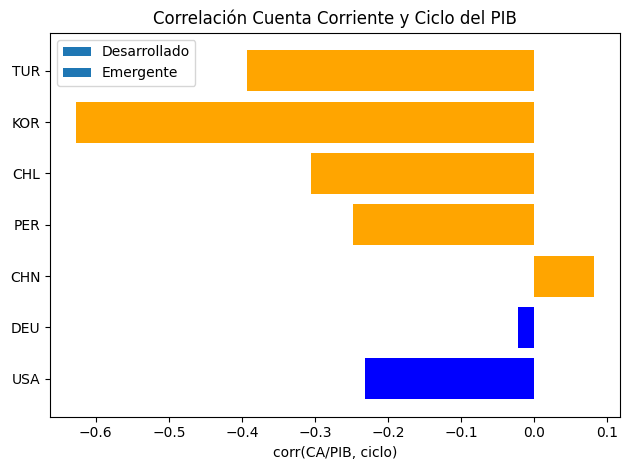
\includegraphics[width=0.8\textwidth]{grafico_item22.png}
\caption{Correlación entre cuenta corriente y ciclo del producto por país}
\end{figure}

\section*{Ítem 23}

\subsection*{(a)}
R2 se cumple en todos los países menos China, pues este último tiene una corr con CA positiva (+0.082). El promedio (en valor absoluto) de R2 en economías desarrolladas es de 0.127, mientras que en emergentes es 0.331. Esto confirma que la CA es más cotracíclica en economías emergentes.
Si se puede ver un patrón, en las economías emergentes, la mayor contraciclidad en la CA indica que la inversión es la referente en los ajustes ante shocks. En cambio, en economías desarrolladas se muestra un suavizamiento del consumo. Esto hace sentido pues las economías desarrolladas tienen un mejor acceso a los sistemas financieros internacionales, que permite tener un endeudamiento prolongado.


\subsection*{(b)}
R6 no se cumple para Alemania (tiene un valor -0.265). Chile tiene un R6 positivo pero bastante bajo.
Cuando S-I es bajo, el ahorro doméstico y la inversión no se vinculan fuertemente. Esto significa que el país puede ahorrar en el exterior o financiar su inversión con capital del exterior. Por lo tanto, el valor bajo de S-I si sugiere que el país esté más integrado en el sistema financiero internacional (y mayoe movilidad de capitales).


\subsection*{(c)}
R5 falla para Alemania (1.637) y Corea (1.773), eso indica que la inversión es más volatil que el consumo. En los demás países se da el caso contrario. Las economías que muestran el comportamiento más volatil en el consumo suelen ser emergentes (es curioso que esté EE.UU.), pues estas presentan mayores problemas para suavizar el consumo, puede ser por el limitado acceso al crédito, y su sensibilidad es mayor ante shocks.


El primer país que no coincide con la teoría inicial es EE.UU., esto puede deberse a lo relevante que es el dólar a nivel mundial como moneda de reserva. Esta gran demanda por la moneda da un buen espacio a EE.UU. para financiar sus desequlibrios externos facilmente.
El segundo país que no coincide con la teoría es Chile. Este país usa sus fondos soberanos para obtener una política contracíclica y suavizar la inversión pública. Además, es un país afectado por los shocks detérminos de intercambio (precio del cobre mayormente), esto hace que el ingreso nacional tenga una mayor fluctuación y el conusumo sea impactado.


\section*{Ítem 24}

En la economía sin inversión no existe acumulación, los agentes ahorran en momentos positivos y desahorran en una recesión. Por lo tanto, se puede observar comportamiento procíclico en cuanto a la CA. Asimismo, va de acorde al comportamiento de R1

En la economía con inversión, en cambio, cuando hay un shock de productividad, por ejemplo, y la demanda por capital (para invertir) aumenta, lo que genera deficits externos y, por consecuencia, reducir la CA (contracíclica). Esto va de acorde al comportamiento de R2.

R1 se asocia con la CA procíclica (aquí se da el suavizamiento de consumo) y R2 se asocia con la CA contracíclica (acumulación de capital), por lo tanto, el canal que se encuentra apagado en una economía de dotaciones es el de inversión (acumulación de capital).

corr(CA/PIB, ciclo) con inversion = -0.033
corr(CA/PIB, ciclo) sin inversion = +0.318

\begin{figure}[H]
\centering
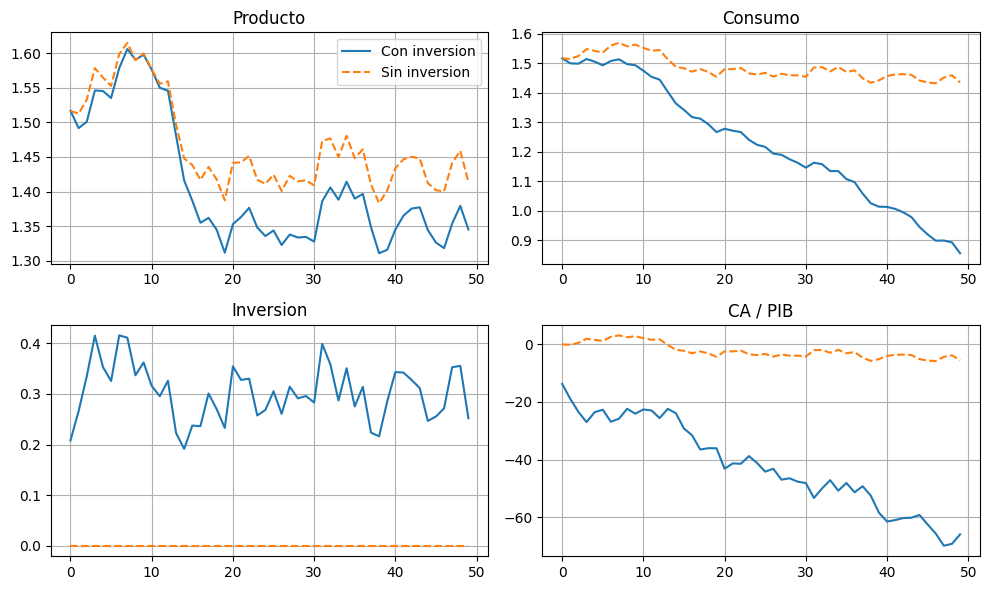
\includegraphics[width=0.8\textwidth]{grafico_item24.png}
\caption{Comparación de dinámicas con y sin inversión}
\end{figure}

\section*{Ítem 25}

\begin{table}[H]
\centering
\caption{Efectos de cambios paramétricos sobre inversión y cuenta corriente}
\begin{tabular}{cccc}
\toprule
Parámetro & Cambio & $\Delta I$ & $\Delta CA$ \\
\midrule
$\rho$ & $\uparrow$ & $\uparrow$ & $\downarrow$ \\
$\alpha$ & $\uparrow$ & $\uparrow$ & $\downarrow$ \\
$r^*$ & $\uparrow$ & $\downarrow$ & $\uparrow$ \\
$\sigma_{\epsilon}$ & $\uparrow$ & $\uparrow$ & $\downarrow$ \\
$\beta$ & $\uparrow$ & $\uparrow$ & $\uparrow$ \\
\bottomrule
\end{tabular}
\end{table}

\begin{table}[H]
\centering
\caption{Intuición económica de los cambios paramétricos}
\begin{tabular}{p{2cm} p{11cm}}
\toprule
Parámetro & Intuición \\
\midrule
$\rho$ & Como shock es más persistente, el retorno esperado de capital es elevado y se incentiva a invertir hoy, esto incrementa el déficit externo \\

$\alpha$ & Mayor peso de capital eleva la productividad marginal, aumenta inversion y mayor déficit en CA \\

$r^*$ & Mayor costo de financia. desincentiva inversión y reduce endeudamiento externo, por lo que CA aumenta\\

$\sigma_{\epsilon}$ & Shocks generan mayor fluctuacion en inversion, se amplifican los deficits y superavits externos \\

$\beta$ & Agentes más pacientes ahorran más, reduce la necesidad de financiarse y modera el deficit de CA \\
\bottomrule
\end{tabular}
\end{table}


\section*{Ítem 26}

\subsection*{Paso 1}

Se aumentó $\rho$, $\alpha$ y $\sigma_\epsilon$, y se redujo $r^*$ para mejorar los momentos del modelo.

\begin{table}[H]
\centering
\caption{Comparación de momentos: modelo base vs calibrado}
\begin{tabular}{lccc}
\toprule
Momento & Base & Calibrado \\
\midrule
corr(CA, ciclo) & 0.012 & 0.011 \\
corr(I, ciclo) & 0.634 & 0.551 \\
$\sigma(I)/\sigma(C)$ & 0.012 & 0.059 \\
\bottomrule
\end{tabular}
\end{table}

\subsection*{Paso 3}

Simular-economía es una versión muy simple de una economia abierta. El paper incorpora shocks en los términos de cambios (como el cobre) que afectan directamente en la CA. También desgrega el gasto, lo que mueve bastante la dinámica entre el consumo y la inversion. Además, el paper incorpora un ambiente de dinámica inflacionaria y política monetaria que no se encuentran en este sencillo modelo.  Los criterios del paper permiten modelar de forma más empírica sin la necesidad de ajustar demasiado los parámetros.

\end{document}

\end{document}